\documentclass[xcolor={table}]{beamer}
\PassOptionsToPackage{cmyk}{xcolor}
\usefonttheme{professionalfonts}
\usefonttheme{serif}
\usepackage{natbib}
\usepackage{times}
\usepackage{tabularx}
\usepackage{ulem}
\usepackage{color,soul}
\usepackage[table]{xcolor}
\usepackage{tikz}
\usetikzlibrary{calc}
\usepackage{graphicx,import}
\usepackage{tcolorbox}
\usepackage{bbm}

\makeatletter
\newcommand\SoulColor{%
    \let\set@color\beamerorig@set@color
    \let\reset@color\beamerorig@reset@color}
\makeatother

\definecolor{conc}{HTML}{660000}
\definecolor{proc}{HTML}{194f19}
\newcommand\conit[1]{\item[\textcolor{conc}{$-$}] \textcolor{conc}{#1}}
\newcommand\proit[1]{\item[\textcolor{proc}{$+$}] \textcolor{proc}{#1}}
\newcommand\spit{\hspace{\labelwidth}}

\newcommand\nodecite[1]{\fontsize{9.2pt}{12pt}\selectfont\citet{#1}}
\newcommand\nodeciteh[1]{\fontsize{9.2pt}{12pt}\selectfont\textcolor{proc}{
    \citet{#1}}}


\newcommand\Wider[2][3em]{%
\makebox[\linewidth][c]{%
  \begin{minipage}{\dimexpr\textwidth+#1\relax}
  \raggedright#2
  \end{minipage}%
  }%
}


\usetheme{metropolis}           % Use metropolis theme
\title{Automatic Summarization: Evaluation, Extraction, and Abstraction}
\date{\today}
\author{Chris Kedzie}
\institute{Dept. of Computer Science, Columbia University}
\begin{document}
  \maketitle


\begin{frame}{Presentation Overview}

\begin{enumerate}
    \item \textbf{Task Definition \& Variations}
        ~\\~\\
    \item \textbf{Evaluation}
        ~\\~\\
    \item \textbf{Two Implementation Paradigms}
\begin{enumerate}
\item Extractive Summarization
\item Abstractive Summarization
\end{enumerate}
\end{enumerate}

\end{frame}


\section{Summarization Task}




\begin{frame}{Summarization Tasks}
\only<1>{\resizebox{\textwidth}{!}{\Huge{\import{svg/}{tasks1.pdf_tex}}}}
\only<2>{\resizebox{\textwidth}{!}{\Huge{\import{svg/}{tasks2.pdf_tex}}}}
\only<3>{\resizebox{\textwidth}{!}{\Huge{\import{svg/}{tasks3.pdf_tex}}}}
\only<4>{\resizebox{\textwidth}{!}{\Huge{\import{svg/}{tasks4.pdf_tex}}}}
\only<5>{\resizebox{\textwidth}{!}{\Huge{\import{svg/}{tasks5.pdf_tex}}}}
\end{frame}





\section{Evaluation}

\begin{frame}{Summary Evaluation: Document Understanding Conf.}
  
  ~\\
  
  \textbf{Linguistic Quality}
  \begin{itemize}
    \small
    \item Are the summaries grammatical, coherent, and otherwise well written?
  \end{itemize}

  ~\\~\\

  \textbf{Content Selection}
  \begin{itemize}
    \small
    \item Do they convey the important information in the input documents?
  \end{itemize}
\end{frame}


\begin{frame}{Content Selection Evaluation: Document Understanding Conf.}

  ~\\

  {\large\textbf{Coverage Assessment}}
  {\footnotesize\textbf{(DUC 01-04)}}
  \begin{itemize}
    \small
    \item How much of the meaning in a reference summary is covered by the\\
        \spit system summary? (6 pt. scale)
    \uncover<2->{\conit{Judgement made with only 1 reference summary!}}
    \uncover<3->{\conit{Coverage assessor often the author of the reference!}}
  \end{itemize}

  ~\\

  {\large\textbf{Responsiveness Assessment} }
  {\footnotesize\textbf{(DUC 03-07, TAC 08-11)}} 
  \begin{itemize}
    \small
    \item  How well does a summary answer the information need, given the\\ 
        \spit topic query/user profile? (5 pt. scale)
    \uncover<4->{\proit{No reference summary needed!}}
  \end{itemize}
\end{frame}

\begin{frame}{Content Evaluation Road Map}
 \Wider[4.1em]{
  \begin{figure}[h]
   \centering
   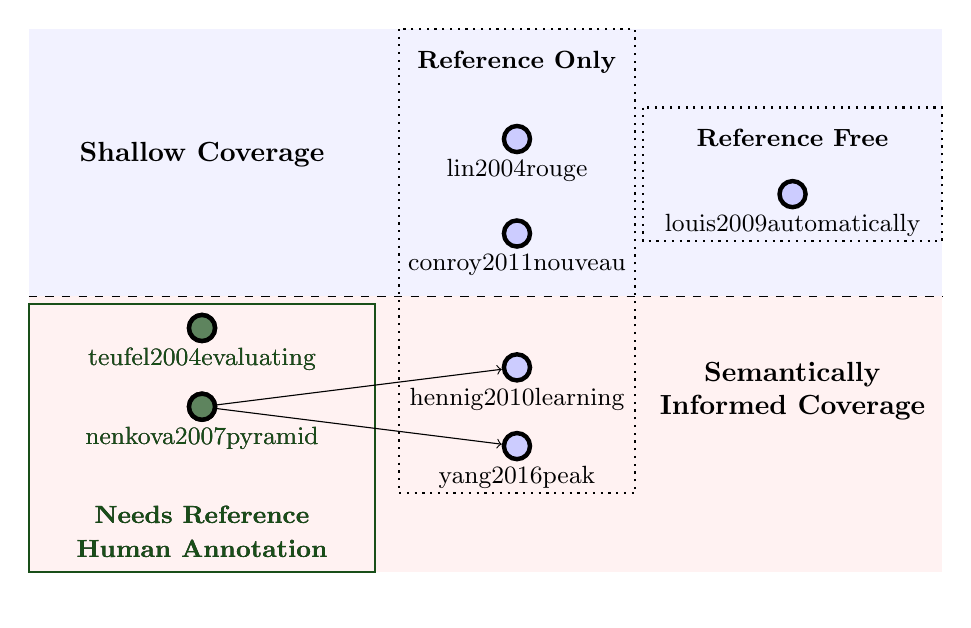
\begin{tikzpicture}[
     dep/.style={draw, shape=circle, ultra thick, fill=blue!20},
     depa/.style={draw, shape=circle, ultra thick, fill=proc!70},
   ]
 
    \draw[fill=none,draw=none] (-2,1.6) rectangle (8,-5.3);
    \visible<2->{
     \draw[fill=blue!5,draw=none] (-3.2, 1.6) rectangle (8.4,-1.8);
     \draw[fill=red!5,draw=none]  (-3.2,-5.3) rectangle (8.4,-1.8);
     \draw[dashed] (-3.2,-1.8) -- (8.4,-1.8);

     \node at (-1,0) {\textbf{Shallow Coverage}};
     \node[align=center] at (6.5,-3.0) 
      {\textbf{Semantically}\\
       \textbf{Informed Coverage}
      };
    }
 
    \visible<3>{
     \draw[thick,dotted] (-3.2,-1.9) rectangle (1.2,-5.3);
     \node[align=center] (x) at (-1,-5) {
        \small \textbf{Needs Reference}\\
        \small \textbf{Human Annotation}\\};
    } 
    \visible<3->{
     \draw[thick,dotted] (1.5,1.6) rectangle (4.5,-4.3);
     \node[align=center] (y) at (3,1) {\small \textbf{Reference Only}\\};
     \draw[thick,dotted] (4.6,0.6) rectangle (8.4,-1.1);
     \node[align=center] (z) at (6.5,0) {\small \textbf{Reference Free}\\};
    }
 
    \node[dep] (linnode) at (3,.2) {};
    \node[] (lintxt) at (3,-.2) {\nodecite{lin2004rouge}};
    \node[dep] (conroynode) at (3,-1) {};
    \node[] (conroytxt) at (3,-1.4) {\nodecite{conroy2011nouveau}};
 
    \node[dep] (teufelnode) at (-1,-2.2) {};
    \node[] (teufeltxt) at (-1,-2.6) {\nodecite{teufel2004evaluating}};
    \node[dep] (nenkovanode) at (-1,-3.2) {};
    \node[] (nenkovatxt) at (-1,-3.6) {\nodecite{nenkova2007pyramid}};
 
    \visible<4->{
     \node[depa] (teufelnode) at (-1,-2.2) {};
     \node[depa] (nenkovanode) at (-1,-3.2) {};
     \draw[thick,draw=proc] (-3.2,-1.9) rectangle (1.2,-5.3);
     \node[] (teufeltxt) at (-1,-2.6) {\nodeciteh{teufel2004evaluating}};
     \node[] (nenkovatxt) at (-1,-3.6) {\nodeciteh{nenkova2007pyramid}};
 
     \node[align=center] (x) at (-1,-5) {
         \small\textcolor{proc}{\textbf{Needs Reference}}\\
         \small\textcolor{proc}{\textbf{Human Annotation}}\\
     };
    }

    \node[dep] (hennignode) at (3,-2.7) {};
    \node[] (hennigtxt) at (3,-3.1) {\nodecite{hennig2010learning}};
    \node[dep] (yangnode) at (3,-3.7) {};
    \node[] (yangtxt) at (3,-4.1) {\nodecite{yang2016peak}};

    \node[dep] (louisnode) at (6.5,-.5) {};
    \node[] (louistxt) at (6.5, -.9) {\nodecite{louis2009automatically}};
    \path [->] (nenkovanode) edge (hennignode); 
    \path [->] (nenkovanode) edge (yangnode); 

   \end{tikzpicture}
  \end{figure}
 }
\end{frame}

\begin{frame}[t]{Factoids and Pyramids}
  \textbf{Factoids} {\small \citep{teufel2004evaluating}} \\
  \textbf{Pyramid} {\small \citep{nenkova2007pyramid} }
  \begin{itemize}
    \small
    \item Label factoids/SCUs in ref. summaries.
    \uncover<3->{\item Weight factoids/SCUs by frequency in references.}
    \uncover<4->{\item Summary score $\propto$ to the sum of weights of 
        factoids/SCUs contained.}
    \uncover<5->{\proit{More reliable assessment than ``coverage score'' 
                 procedure! }}
  \end{itemize}
 
  ~\\
  \only<1-4>{        
  \uncover<2-4>{\small SCU label: \textit{Lopez left GM for VW}\\} 
  \uncover<3-4>{\small SCU Weight: 2\\}
  }

  \only<1-4>{
   \uncover<2-4>{
    \begin{itemize}
      \scriptsize
      \item
        The industrial espionage case involving GM and VW began with 
        \SoulColor\hl{the} \SoulColor\hl{hiring of Jose Ignacio Lopez, an 
        employee of GM} subsidiary Adam Opel, \SoulColor\hl{by VW} as a 
        production director.
  
      \item
         However, \SoulColor\hl{he left GM for VW} under circumstances, which 
         along with ensuing events, were described by a German judge as 
         ``potentially the biggest ever case of industrial espionage.''
    \end{itemize}
   }
  }
  \only<5->{
  \uncover<6->{
     Disagreement in annotator stability:
     \begin{itemize}
       \small
       \conit{Factoids require 20-30 reference summaries! 
                {\scriptsize\citep{teufel2004evaluating}}}
         \proit{Pyramid requires at least 5 reference summaries!
             {\scriptsize\citep{nenkova2007pyramid}}}
        \proit{Pyramid requires at least 2-3 reference summaries 
                for correlation with responsiveness!
             {\scriptsize\citep{owczarzak2009evaluation}}}
         
     \end{itemize}
  }}
\end{frame}
 
\begin{frame}{Content Evaluation Road Map}
 \Wider[4.1em]{
  \begin{figure}[h]
   \centering
   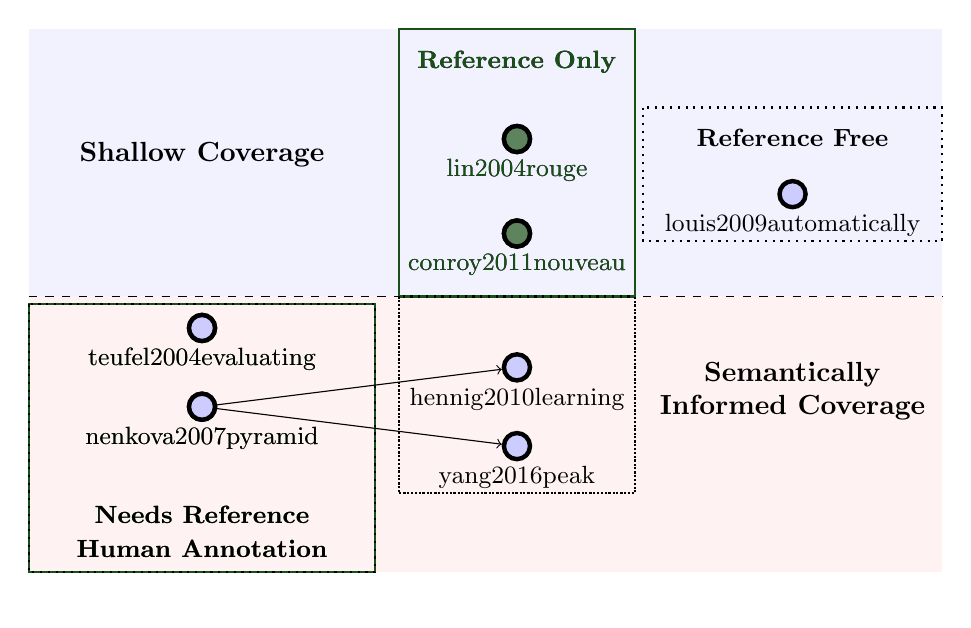
\begin{tikzpicture}[
     dep/.style={draw, shape=circle, ultra thick, fill=blue!20},
     depa/.style={draw, shape=circle, ultra thick, fill=proc!70},
   ]

    \draw[fill=none,draw=none] (-3.2,1.6) rectangle (8.4,-5.3);
    \draw[fill=blue!5,draw=none] (-3.2,1.6) rectangle (8.4,-1.8);
    \draw[fill=red!5,draw=none] (-3.2,-5.3) rectangle (8.4,-1.8);
    \draw[dashed] (-3.2,-1.8) -- (8.4,-1.8);

    \node at (-1,0) {\textbf{Shallow Coverage}};
    \node[align=center] at (6.5,-3.0) 
        {\textbf{Semantically}\\
         \textbf{Informed Coverage}
        };

    \visible<1>{
     \node[align=center] at (-1,-5) {
         \small \textcolor{proc}{\textbf{Needs Reference}}\\
         \small \textcolor{proc}{\textbf{Human Annotation}}\\};
     \node[depa] (teufelnode) at (-1,-2.2) {};
     \node[depa] (nenkovanode) at (-1,-3.2) {};
     \draw[thick,draw=proc] (-3.2,-1.9) rectangle (1.2,-5.3);
     \node[] (teufeltxt) at (-1,-2.6) {\nodeciteh{teufel2004evaluating}};
     \node[] (nenkovatxt) at (-1,-3.6) {\nodeciteh{nenkova2007pyramid}};
    }
    \visible<2->{
     \draw[thick,dotted] (-3.2,-1.9) rectangle (1.2,-5.3);
     \node[align=center] at (-1,-5) {
         \small \textbf{Needs Reference}\\
         \small \textbf{Human Annotation}\\};
     \node[dep] (teufelnode) at (-1,-2.2) {};
     \node[dep] (nenkovanode) at (-1,-3.2) {};
     \node[] (teufeltxt) at (-1,-2.6) {\nodecite{teufel2004evaluating}};
     \node[] (nenkovatxt) at (-1,-3.6) {\nodecite{nenkova2007pyramid}};
    }

    \visible<-2>{
     \draw[thick,dotted] (1.5,1.6) rectangle (4.5,-4.3);
     \node[align=center] (y) at (3,1) {\small \textbf{Reference Only}\\};
     \node[dep] (linnode) at (3,.2) {};
     \node[] (lintxt) at (3,-.2) {\nodecite{lin2004rouge}};
     \node[dep] (conroynode) at (3,-1) {};
     \node[] (conroytxt) at (3,-1.4) {\nodecite{conroy2011nouveau}};
 
    }
    \visible<3>{
     \node[align=center] at (3,1) {
        \small \textcolor{proc}{\textbf{Reference Only}}\\};
     \node[depa] (linnode) at (3,.2) {};
     \node[] (lintxt) at (3,-.2) {\nodeciteh{lin2004rouge}};
     \node[depa] (conroynode) at (3,-1) {};
     \node[] (conroytxt) at (3,-1.4) {\nodeciteh{conroy2011nouveau}};
     \draw[thick,draw=proc] (1.5,1.6) rectangle (4.5,-1.8);
     \draw[thick,dotted] (1.5,-1.8) rectangle (4.5,-4.3);
    }

    \node[dep] (hennignode) at (3,-2.7) {};
    \node[] (hennigtxt) at (3,-3.1) {\nodecite{hennig2010learning}};
    \node[dep] (yangnode) at (3,-3.7) {};
    \node[] (yangtxt) at (3,-4.1) {\nodecite{yang2016peak}};
    \node[dep] (louisnode) at (6.5,-.5) {};
    \node[] (louistxt) at (6.5, -.9) {\nodecite{louis2009automatically}};
    \path [->] (nenkovanode) edge (hennignode); 
    \path [->] (nenkovanode) edge (yangnode); 
    \draw[thick,dotted] (4.6,0.6) rectangle (8.4,-1.1);
    \node[align=center] (z) at (6.5,0) {\small \textbf{Reference Free}\\};

   \end{tikzpicture}
  \end{figure}
 }
\end{frame}

\begin{frame}{Reference Only, Shallow Coverage}

 \textbf{ROUGE }{\small\citep{lin2004rouge}} -- recall of reference summary 
    ngrams
 \begin{itemize}
        \small
   \item De facto standard evaluation tool outside of DUC/TAC.
   \conit{Insensitive to semantics/synonomy.}
   \conit{Correlation with coverage is only strong at 200 and 400 word 
        length!\\
    \spit {\scriptsize \citep{lin2004rouge,nenkova2005automatic}}}
   \proit{Strong rank correlation with responsiveness  
          and pyramid (R2 $>$ .87)!\\
    \spit {\scriptsize \citep{louis2009automatically,owczarzak2009evaluation}}}
 \end{itemize}
 \textbf{Nouveau ROUGE} {\small\citep{conroy2011nouveau}} -- 
        {\small{(Update Summarization)}}\\ \spit Penalize for high ROUGE score
        on background set summary. 
 \begin{itemize}
     \small
     \proit{Makes relationship between ROUGE and 
                pyramid/responsiveness\\ \spit more linear.}
 \end{itemize}
\end{frame}

\begin{frame}{Content Evaluation Road Map}
 \Wider[4.1em]{
  \begin{figure}[h]
   \centering
   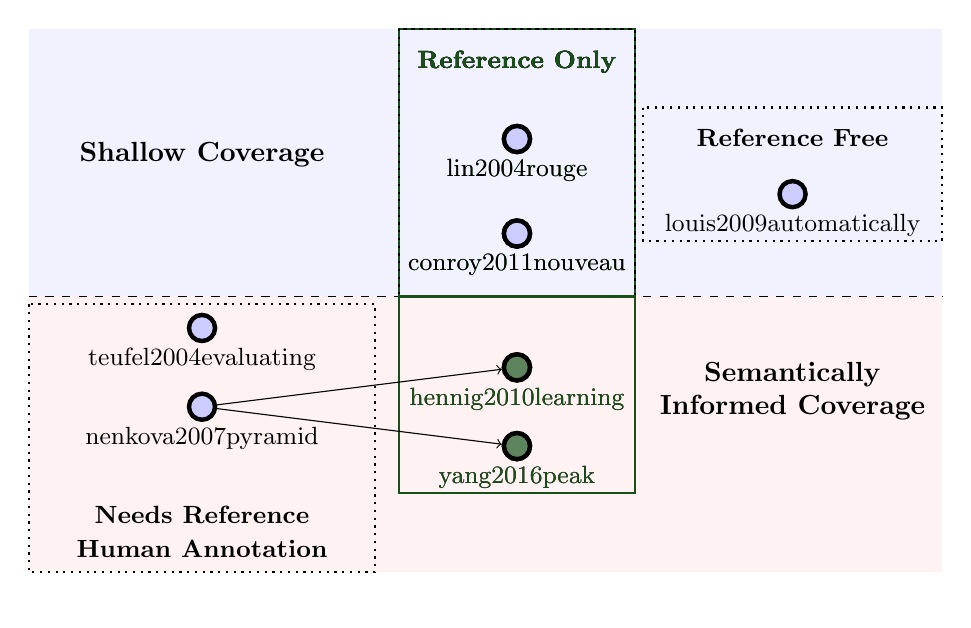
\begin{tikzpicture}[
     dep/.style={draw, shape=circle, ultra thick, fill=blue!20},
     depa/.style={draw, shape=circle, ultra thick, fill=proc!70},
   ]
 
    \draw[fill=none,draw=none] (-3.2,1.6) rectangle (8.4,-5.3);
    \draw[fill=blue!5,draw=none] (-3.2, 1.6) rectangle (8.4,-1.8);
    \draw[fill=red!5,draw=none]  (-3.2,-5.3) rectangle (8.4,-1.8);
    \draw[dashed] (-3.2,-1.8) -- (8.4,-1.8);

    \node at (-1,0) {\textbf{Shallow Coverage}};
    \node[align=center] at (6.5,-3.0) 
      {\textbf{Semantically}\\
       \textbf{Informed Coverage}
      };
    \draw[thick,dotted] (-3.2,-1.9) rectangle (1.2,-5.3);
    \node[align=center] at (-1,-5) {
        \small \textbf{Needs Reference}\\
        \small \textbf{Human Annotation}\\};

    \node[align=center] (y) at (3,1) {\small \textbf{Reference Only}\\};
    \draw[thick,dotted] (4.6,0.6) rectangle (8.4,-1.1);
    \node[align=center] (z) at (6.5,0) {\small \textbf{Reference Free}\\};

    \visible<1>{
     \node[depa] (linnode) at (3,.2) {};
     \node[] (lintxt) at (3,-.2) {\nodeciteh{lin2004rouge}};
     \node[depa] (conroynode) at (3,-1) {};
     \node[] (conroytxt) at (3,-1.4) {\nodeciteh{conroy2011nouveau}};
     \node[align=center] (y) at (3,1) 
        {\small \textcolor{proc}{\textbf{Reference Only}}\\};
     \draw[thick,draw=proc] (1.5,1.6) rectangle (4.5,-1.8);
     \draw[thick,dotted] (1.5,-1.8) rectangle (4.5,-4.3);
    }
    \visible<-2>{
     \node[dep] (hennignode) at (3,-2.7) {};
     \node[] (hennigtxt) at (3,-3.1) {\nodecite{hennig2010learning}};
     \node[dep] (yangnode) at (3,-3.7) {};
     \node[] (yangtxt) at (3,-4.1) {\nodecite{yang2016peak}};
    }
    \visible<2->{
     \node[dep] (linnode) at (3,.2) {};
     \node[] (lintxt) at (3,-.2) {\nodecite{lin2004rouge}};
     \node[dep] (conroynode) at (3,-1) {};
     \node[] (conroytxt) at (3,-1.4) {\nodecite{conroy2011nouveau}};
    } 
    \visible<2>{
     \node[align=center] at (3,1) 
        {\small \textbf{Reference Only}\\};
     \draw[thick,dotted] (1.5,1.6) rectangle (4.5,-4.3);
    }
    \visible<3>{
     \node[align=center] at (3,1) 
        {\small \textcolor{proc}{\textbf{Reference Only}}\\};
     \draw[thick,dotted] (1.5,1.6) rectangle (4.5,-1.8);
     \draw[thick,draw=proc] (1.5,-1.8) rectangle (4.5,-4.3);
     \node[depa] (hennignode) at (3,-2.7) {};
     \node[] (hennigtxt) at (3,-3.1) {\nodeciteh{hennig2010learning}};
     \node[depa] (yangnode) at (3,-3.7) {};
     \node[] (yangtxt) at (3,-4.1) {\nodeciteh{yang2016peak}};
    }



    \node[dep] (teufelnode) at (-1,-2.2) {};
    \node[] (teufeltxt) at (-1,-2.6) {\nodecite{teufel2004evaluating}};
    \node[dep] (nenkovanode) at (-1,-3.2) {};
    \node[] (nenkovatxt) at (-1,-3.6) {\nodecite{nenkova2007pyramid}};
 
    \node[dep] (louisnode) at (6.5,-.5) {};
    \node[] (louistxt) at (6.5, -.9) {\nodecite{louis2009automatically}};
    \path [->] (nenkovanode) edge (hennignode); 
    \path [->] (nenkovanode) edge (yangnode); 

   \end{tikzpicture}
  \end{figure}
 }
\end{frame}

\begin{frame}{Automating Pyramid}

 \textbf{LDA} {\scriptsize\citep{hennig2010learning}} -- topics $\approx$ SCU
 \begin{itemize}
        \small
  \item LDA topics and SCU's unigram distributions are very similar. 
  \only<1>{\item Good matching between LDA topics and SCUs is possible.}
  \only<2->{\proit{Good matching between LDA topics and SCUs is 
        possible.}}
  \only<-2>{\item Theoretical, no method yet of selecting appropriate 
        topics w/o SCUs.}
  \only<3->{\conit{Theoretical, no method yet of selecting 
        appropriate topics w/o SCUs.}}
 \end{itemize}

 \textbf{PEAK} {\scriptsize\citep{yang2016peak}} -- subj-pred.-obj tuple $\approx$ SCU

 \begin{itemize}
   \small
   \item Uses Open-IE style pattern extraction as stand-in for SCU's.
   \item System SCU's mapped to Reference SCU's via maximal matching.
   \only<-3>{\item (DUC 06) Moderate correlation with pyramid scores (.7094).}
   \only<4->{\proit{(DUC 06) Moderate correlation with pyramid 
        scores (.7094).}}
   \only<-4>{\item Unclear if the rank correlation is higher than ROUGE-2.}
   \only<5>{\conit{Unclear if the rank correlation is higher than 
        ROUGE-2.}}
 \end{itemize}
\end{frame}

\begin{frame}{Content Evaluation Road Map}
 \Wider[4.1em]{
  \begin{figure}[h]
   \centering
   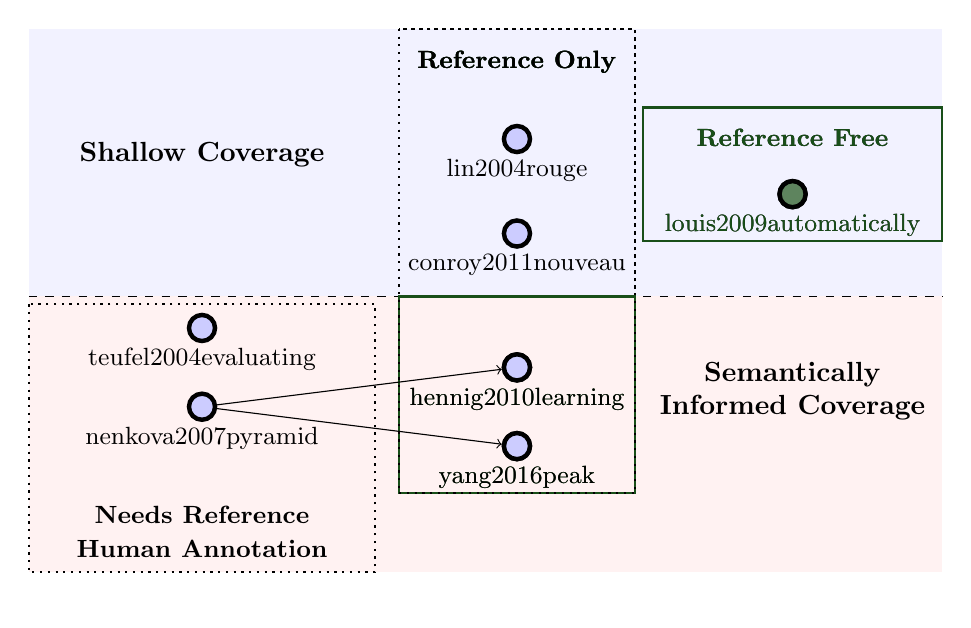
\begin{tikzpicture}[
     dep/.style={draw, shape=circle, ultra thick, fill=blue!20},
     depa/.style={draw, shape=circle, ultra thick, fill=proc!70},
   ]
 
    \draw[fill=none,draw=none] (-3.2,1.6) rectangle (8.4,-5.3);
    \draw[fill=blue!5,draw=none] (-3.2, 1.6) rectangle (8.4,-1.8);
    \draw[fill=red!5,draw=none]  (-3.2,-5.3) rectangle (8.4,-1.8);
    \draw[dashed] (-3.2,-1.8) -- (8.4,-1.8);

    \node at (-1,0) {\textbf{Shallow Coverage}};
    \node[align=center] at (6.5,-3.0) 
      {\textbf{Semantically}\\
       \textbf{Informed Coverage}
      };
    \draw[thick,dotted] (-3.2,-1.9) rectangle (1.2,-5.3);
    \node[align=center] at (-1,-5) {
        \small \textbf{Needs Reference}\\
        \small \textbf{Human Annotation}\\};

    \node[align=center] (y) at (3,1) {\small \textbf{Reference Only}\\};


    \visible<1>{
     \node[align=center] at (3,1) 
        {\small \textcolor{proc}{\textbf{Reference Only}}\\};
     \draw[thick,dotted] (1.5,1.6) rectangle (4.5,-1.8);
     \draw[thick,draw=proc] (1.5,-1.8) rectangle (4.5,-4.3);
     \node[depa] (hennignode) at (3,-2.7) {};
     \node[] (hennigtxt) at (3,-3.1) {\nodeciteh{hennig2010learning}};
     \node[depa] (yangnode) at (3,-3.7) {};
     \node[] (yangtxt) at (3,-4.1) {\nodeciteh{yang2016peak}};
    }
    \visible<2->{
     \draw[thick,dotted] (1.5,1.6) rectangle (4.5,-4.3);
     \node[align=center] at (3,1) 
        {\small \textbf{Reference Only}\\};
     \node[dep] (hennignode) at (3,-2.7) {};
     \node[] (hennigtxt) at (3,-3.1) {\nodecite{hennig2010learning}};
     \node[dep] (yangnode) at (3,-3.7) {};
     \node[] (yangtxt) at (3,-4.1) {\nodecite{yang2016peak}};
    }

    \visible<-2>{
     \node[dep] (louisnode) at (6.5,-.5) {};
     \node[] (louistxt) at (6.5, -.9) {\nodecite{louis2009automatically}};
     \draw[thick,dotted] (4.6,0.6) rectangle (8.4,-1.1);
     \node[align=center] at (6.5,0) {\small \textbf{Reference Free}\\};
    }
    \visible<3>{
     \node[depa] (louisnode) at (6.5,-.5) {};
     \node[] (louistxt) at (6.5, -.9) {\nodeciteh{louis2009automatically}};
     \draw[thick,draw=proc] (4.6,0.6) rectangle (8.4,-1.1);
     \node[align=center] at (6.5,0) 
        {\small \textcolor{proc}{\textbf{Reference Free}}\\};
    }

    \node[dep] (linnode) at (3,.2) {};
    \node[] (lintxt) at (3,-.2) {\nodecite{lin2004rouge}};
    \node[dep] (conroynode) at (3,-1) {};
    \node[] (conroytxt) at (3,-1.4) {\nodecite{conroy2011nouveau}};
    \node[dep] (teufelnode) at (-1,-2.2) {};
    \node[] (teufeltxt) at (-1,-2.6) {\nodecite{teufel2004evaluating}};
    \node[dep] (nenkovanode) at (-1,-3.2) {};
    \node[] (nenkovatxt) at (-1,-3.6) {\nodecite{nenkova2007pyramid}};
    \path [->] (nenkovanode) edge (hennignode); 
    \path [->] (nenkovanode) edge (yangnode); 

   \end{tikzpicture}
  \end{figure}
 }
\end{frame}



\begin{frame}{Evaluation without Human Models}
\textbf{\cite{louis2009automatically}} \\
Examines correlation between
    input/summary 
    features and TAC08 responsiveness and pyramid scores.
 \begin{itemize}
        \small
    \proit{(Across systems) Jensen-Shannon (JS) divergence correlated 
        with} 
    \begin{figure}[h]
     \centering
     \begin{tabular}{| l | l |}       
      \hline
      Pyramid $-.88$ & Responsiveness. $-.74$  \\
      \hline
     \end{tabular}
    \end{figure}
    \conit{(Within topics) Correlations vary widely per document set.}
    \only<1>{\item Establishing system rankings seems possible w/o references}
    \only<2->{\proit{Establishing system rankings seems possible 
        w/o references}}
    \only<-2>{\item Unclear what would happen if JS div. explicitly minimized.}
    \only<3>{\conit{Unclear what would happen if JS div. explicitly minimized.}}
 \end{itemize}
\end{frame}


\begin{frame}{Summary Evaluation}

    \begin{itemize}
        \item Research focus on content selection evaluation: \\
            Pyramid, Factoid, ROUGE
            ~\\~\\
        \proit{Despite flaws, ROUGE-2 is simple and highly correlated with 
            human metrics}
            ~\\~\\
        \conit{More research is needed on how linguistic quality interacts 
            with content selection scores.}
    \end{itemize}

\end{frame}


\section{Extraction}


\begin{frame}{Extractive Summarization}
    Construct a summary by selecting a subset of sentences (or words) from 
    the inputs.
\end{frame}

\begin{frame}{Extractive Summarization}
  \textbf{Why is extractive summarization so popular?}\\
  ~\\
  \begin{itemize}
    \item Text generation is hard!
    ~\\~\\    
    \item Semantic representations are brittle, low coverage. 
    ~\\~\\
    \item Surface level features (i.e. words) have straightforward \\
           \spit correspondence to ROUGE and human coverage metrics.
    \end{itemize}
\end{frame}

\begin{frame}{Summarization in Different Domains}
  \uncover<2>{{\large\textbf{Retrospective Summarization}}}
  \begin{itemize}
    \item[] 
\includegraphics[scale=.017]{news_icon}~ \textbf{News} 
      \begin{itemize}
        \item \textit{Text }
            {\fontsize{6.8pt}{12pt}\selectfont\citep{lin2000automated,erkan2004lexrank,conroy2005classy,lin2011class}}
        \item \textit{Broadcast/Speech} {\scriptsize\citep{maskey2005comparing}}
    \end{itemize}
~\\
\item[] 
\includegraphics[scale=.02]{meeting_icon}~ \textbf{Meetings  } 
    {\scriptsize\citep{gillick2009global}}
~\\~\\
\item[] 
\includegraphics[scale=.02]{rating_icon}~ \textbf{Opinions/Reviews} 
    {\scriptsize\citep{titov2008joint}}
~\\~\\
\item[] 
\includegraphics[scale=.02]{tweet_icon}~ \textbf{Microblogs/Twitter} 
    {\scriptsize\citep{liu2011sxsw}}
~\\~\\
    \end{itemize}
    \uncover<2>{
        {\large\textbf{Temporal Summarization}}
    \begin{itemize}
        \item[] 
\includegraphics[scale=.017]{news_icon}~ \textbf{News text} 
        {\scriptsize\citep{guo2013updating,mccreadie2014incremental}}
    \end{itemize}
    }
\end{frame}

  \begin{frame}{
      \only<1>{Extractive Summarization}\only<2>{Extraction by Ranking}}
  \begin{figure}[!h]
    \centering 
    \begin{tikzpicture}
 
      \visible<1>{ 
       \node (C) at (4.7,-1.6) {\textbf{Ranking}};
       \draw[opacity=.2] (4.7,-.6) circle (1.5cm);
       \node at (4.7,.1) {
\includegraphics[scale=.017]{news_icon}};
       \node at (4.7,-.3) {\scriptsize \cite{lin2000automated}};
       \node at (4.7,-.6) {\scriptsize \cite{erkan2004lexrank}};
      }
      \visible<2>{ 
       \node[text=red,opacity=.7] (C) at (4.7,-1.6) {\textbf{Ranking}};
       \draw[opacity=.2,draw=red,opacity=.7] (4.7,-.6) circle (1.5cm);
       \node at (4.7,.1) {
\includegraphics[scale=.022]{news_icon}};
       \node[text=red,opacity=.7] at (4.7,-.3) {\scriptsize \cite{lin2000automated}};
       \node[text=red,opacity=.7] at (4.7,-.6) {\scriptsize \cite{erkan2004lexrank}};
      }

      \node (C) at (3.1,2.5) {
\includegraphics[scale=.017]{news_icon}};
      \node (C) at (3.1,2.0) {\scriptsize \cite{guo2013updating}};
      \node (C) at (3.1,1.7) {\scriptsize \cite{mccreadie2014incremental}};
     
      \node[align=center] (C) at (1.9,5) {\textbf{Classification}\\ 
                                          \textbf{\& Regression}};
      \draw[opacity=.2] (1.9,3) circle (2.7cm);
      \node (C) at (1.1,4) {
\includegraphics[scale=.017]{news_icon}};
      \node (C) at (1.1,3.6) {\scriptsize\cite{maskey2005comparing}};
      \node (C) at (1.1,3.2) {
\includegraphics[scale=.022]{rating_icon}};
      \node (C) at (1.1,2.8) {\scriptsize\cite{titov2008joint}};
     
      \node (C) at (.5,1.7) {
\includegraphics[scale=.017]{news_icon}};
      \node (C) at (.5,1.3) {\scriptsize\cite{conroy2005classy}};
     
      \node[] (C) at (-.2,-1.6) {\textbf{Optimization}};
      \draw[opacity=.2] (-.2,0.2) circle (2.3cm);
      \node (C) at (-1.2,.4) {
\includegraphics[scale=.017]{tweet_icon}};
      \node (C) at (-1.2,.1) {\scriptsize\cite{liu2011sxsw}};
      \node (C) at (-1.2,-.4) {
\includegraphics[scale=.022]{meeting_icon}};
      \node (C) at (-1.2,-.7) {\scriptsize\cite{gillick2009global}};
      \node (C) at (.8,0) {
\includegraphics[scale=.017]{news_icon}};
      \node (C) at (.8,-.3) {\scriptsize\cite{lin2011class}};
      
   \end{tikzpicture}
 \end{figure}
\end{frame}

\begin{frame}{Extraction by Ranking}
    \begin{enumerate}
        \item Apply a ranking over sentences, and 
            ~\\
            ~\\
            ~\\
        \item greedily add the top sentences,\\
            \spit stopping when length
            constraint is reached.
    \end{enumerate}

\end{frame}

\begin{frame}[t]{Extraction by Ranking}
    \begin{itemize}
        \uncover<2->{\item \textbf{Centroid Similarity} Cosine similarity of tf$\cdot$idf vector to the mean input tf$\cdot$idf vector.  {\scriptsize \citep{erkan2004lexrank}}}
  \only<2>{
    \begin{figure}[h]
      \centering
      ~\\~\\
      ~\\~\\
      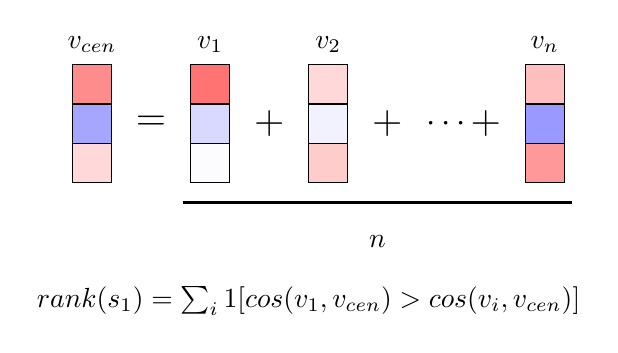
\begin{tikzpicture}
        \draw (0,0) edge (0,1.5);
        \draw (.5,0) edge (.5,1.5);
        \draw (0,0) edge (.5,0);
        \draw (0,.5) edge (.5,.5);
        \draw (0,1) edge (.5,1.0);
        \draw (0,1.5) edge (.5,1.5);
        \draw[fill=red!15] (0,0.5) rectangle (.5,0); 
        \draw[fill=blue!35] (0,1.0) rectangle (.5,.5); 
        \draw[fill=red!45] (0,1.5) rectangle (.5,1.0); 
        \node at (.25,1.75) {$v_{cen}$};
        \node at (1,.75) {\Large $=$};
       
        \draw (1.5,0) edge (1.5,1.5);
        \draw (2,0) edge (2,1.5);
        \draw (1.5,0) edge (2,0);
        \draw (1.50,.5) edge (2,.5);
        \draw (1.50,1) edge (2,1.0);
        \draw (1.50,1.5) edge (2,1.5);
        \draw[fill=blue!1] (1.5,0.5) rectangle (2,0); 
        \draw[fill=blue!15] (1.5,1.0) rectangle (2,.5); 
        \draw[fill=red!55] (1.5,1.5) rectangle (2,1.0); 
        \node at (1.75,1.75) {$v_{1}$};
        \node at (2.5,.75) {\Large $+$};

        \draw (3,0) edge (3,1.5);
        \draw (3.5,0) edge (3.5,1.5);
        \draw (3,0) edge (3.5,0);
        \draw (3,.5) edge (3.5,.5);
        \draw (3,1) edge (3.5,1.0);
        \draw (3,1.5) edge (3.5,1.5);
        \draw[fill=red!20] (3,0.5) rectangle (3.5,0); 
        \draw[fill=blue!5] (3,1.0) rectangle (3.5,.5); 
        \draw[fill=red!15] (3,1.5) rectangle (3.5,1.0); 
        \node at (3.25,1.75) {$v_{2}$};
        \node at (4,.75) {\Large $+$};

        \node at (4.75,.75) {\large $\cdots$};
        \node at (5.25,.75) {\Large $+$};

        \draw (5.75,0) edge (5.75,1.5);
        \draw (6.25,0) edge (6.25,1.5);
        \draw (5.75,0) edge (6.25,0);
        \draw (5.75,.5) edge (6.25,.5);
        \draw (5.75,1) edge (6.25,1.0);
        \draw (5.75,1.5) edge (6.25,1.5);
        \draw[fill=red!40] (5.75,0.5) rectangle (6.25,0); 
        \draw[fill=blue!40] (5.75,1.0) rectangle (6.25,.5); 
        \draw[fill=red!25] (5.75,1.5) rectangle (6.25,1.0); 
        \node at (6,1.75) {$v_{n}$};

        \draw[thick] (1.4,-.25) edge (6.35,-.25);
        \node at (3.875,-.75) {$n$};

        \node at (3,-1.5) 
        {$rank(s_1) = \sum_i \mathbbm{1}[cos(v_1, v_{cen}) > cos(v_i, v_{cen})]$};

        \end{tikzpicture}
      \end{figure}
    }
        \uncover<3->{\item \textbf{Topic Signatures} Rank sentences by number 
            of topically important ngrams. 
            {\scriptsize\citep{lin2000automated}}}
        \only<3>{
  \begin{figure}[h]
    \centering
    ~\\~\\
    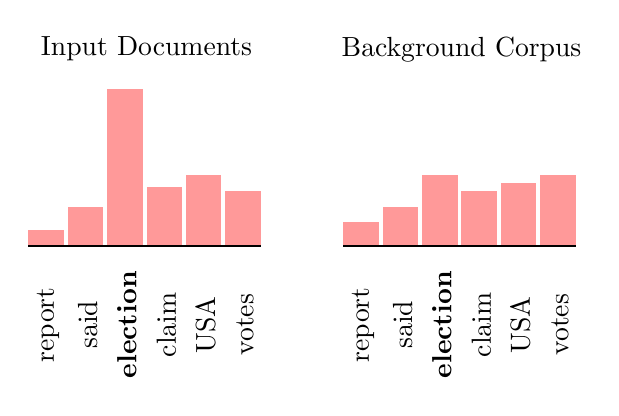
\begin{tikzpicture}
        \draw[fill=red!40,draw=none] (0,.2) rectangle (.45,0);
        \draw[fill=red!40,draw=none] (0.5,.5) rectangle (.95,0);
        \draw[fill=red!40,draw=none] (1,2) rectangle (1.45,0);
        \draw[fill=red!40,draw=none] (1.5,.75) rectangle (1.95,0);
        \draw[fill=red!40,draw=none] (2,.9) rectangle (2.45,0);
        \draw[fill=red!40,draw=none] (2.5,.7) rectangle (2.95,0);
        \node[rotate=90] at (.25,-1) {report};
        \node[rotate=90] at (.75,-1) {said};
        \node[rotate=90] at (1.25,-1) {\textbf{election}};
        \node[rotate=90] at (1.75,-1) {claim};
        \node[rotate=90] at (2.25,-1) {USA};
        \node[rotate=90] at (2.75,-1) {votes};

        \draw[fill=red!40,draw=none] (4,.3) rectangle (4.45,0);
        \draw[fill=red!40,draw=none] (4.5,.5) rectangle (4.95,0);
        \draw[fill=red!40,draw=none] (5,.9) rectangle (5.45,0);
        \draw[fill=red!40,draw=none] (5.5,.7) rectangle (5.95,0);
        \draw[fill=red!40,draw=none] (6,.8) rectangle (6.45,0);
        \draw[fill=red!40,draw=none] (6.5,.9) rectangle (6.95,0);
 
        \node[rotate=90] at (4.25,-1) {report};
        \node[rotate=90] at (4.75,-1) {said};
        \node[rotate=90] at (5.25,-1) {\textbf{election}};
        \node[rotate=90] at (5.75,-1) {claim};
        \node[rotate=90] at (6.25,-1) {USA};
        \node[rotate=90] at (6.75,-1) {votes};

        \draw (0,0) edge (2.95,0);
        \draw (4,0) edge (6.95,0);

        \node at (1.5,2.5) {Input Documents};
        \node at (5.5,2.5) {Background Corpus};
    \end{tikzpicture}
  \end{figure}
}
        \uncover<4->{\item \textbf{LexRank} Rank sentences by graph centrality.
            {\scriptsize \citep{erkan2004lexrank}  }}


    \end{itemize}
     

\only<4->{
~\\~\\
\begin{columns}
    \begin{column}{0.6\textwidth}
        %Content
\centering
        \begin{itemize}
\small
            \item Sentences $\triangleq$ nodes.
            \item Edges determined by cosine similarity.
            \item Rank computed with PageRank.
        \end{itemize}
    \end{column}
    \begin{column}{0.30\textwidth}
\centering
            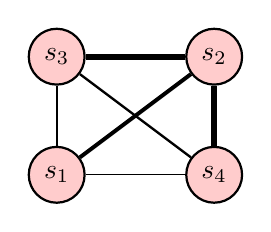
\begin{tikzpicture}[baseline=5ex]
            \node[shape=circle,fill=red!20,thick,draw=black] (1) at (0,0) 
                    {$s_1$};
            \node[shape=circle,fill=red!20,thick,draw=black] (2) at (2,1.5) 
                    {$s_2$};
            \node[shape=circle,fill=red!20,thick,draw=black] (3) at (0,1.5) 
                    {$s_3$};
            \node[shape=circle,fill=red!20,thick,draw=black] (4) at (2,0) 
                    {$s_4$};

                    \path[draw=black,line width=.05cm] (1) -- (2);
                    \path[draw=black,line width=.03cm] (1) -- (3);
                    \path[draw=black] (1) -- (4);
                    \path[draw=black,line width=.08cm] (2) -- (3);
                    \path[draw=black,line width=.07cm] (2) -- (4);
                    \path[draw=black,line width=.03cm] (3) -- (4);


            \end{tikzpicture} 
     \end{column}
\end{columns}
    }  

\end{frame}

\begin{frame}{Extraction by Ranking}
Sentence Ranking Methods:
\begin{itemize}
    \only<1>{\item Simple but effective baselines.}
    \only<2->{\proit{Simple but effective baselines.}}
~\\~\\
    \only<-2>{\item Ranking methods need redundancy penalty/diversity reward
            e.g., MMR.}
    \only<3->{\conit{Ranking methods need redundancy 
        penalty/diversity reward e.g., MMR.}}
~\\~\\
    \only<-3>{\item Ranking implies consistent pairwise ordering \\
        (which definitely does not hold).}
    \only<4>{\conit{Ranking implies consistent pairwise ordering 
            \\ (which definitely does not hold).}}
\end{itemize}
\end{frame}


\begin{frame}{
    \only<1>{Extraction by Ranking}\only<2>{Extractive Summarization}\only<3>{Extraction by Classification \& Regression}}
  \begin{figure}[!h]
    \centering 
    \begin{tikzpicture}
 
      \visible<2->{ 
       \node (C) at (4.7,-1.6) {\textbf{Ranking}};
       \draw[opacity=.2] (4.7,-.6) circle (1.5cm);
       \node at (4.7,.1) {
\includegraphics[scale=.017]{news_icon}};
       \node at (4.7,-.3) {\scriptsize \cite{lin2000automated}};
       \node at (4.7,-.6) {\scriptsize \cite{erkan2004lexrank}};
      }
      \visible<1>{ 
       \node[text=red,opacity=.7] (C) at (4.7,-1.6) {\textbf{Ranking}};
       \draw[opacity=.2,draw=red,opacity=.7] (4.7,-.6) circle (1.5cm);
       \node at (4.7,.1) {
\includegraphics[scale=.022]{news_icon}};
       \node[text=red,opacity=.7] at (4.7,-.3) {\scriptsize \cite{lin2000automated}};
       \node[text=red,opacity=.7] at (4.7,-.6) {\scriptsize \cite{erkan2004lexrank}};
      }

      \visible<-2>{
       \node (C) at (3.1,2.5) {
\includegraphics[scale=.017]{news_icon}};
       \node (C) at (3.1,2.0) {\scriptsize \cite{guo2013updating}};
       \node (C) at (3.1,1.7) {\scriptsize \cite{mccreadie2014incremental}};
     
       \node[align=center] (C) at (1.9,5) {\textbf{Classification}\\ 
                                          \textbf{\& Regression}};
       \draw[opacity=.2] (1.9,3) circle (2.7cm);
       \node (C) at (1.1,4) {
\includegraphics[scale=.017]{news_icon}};
       \node (C) at (1.1,3.6) {\scriptsize\cite{maskey2005comparing}};
       \node (C) at (1.1,3.2) {
\includegraphics[scale=.022]{rating_icon}};
       \node (C) at (1.1,2.8) {\scriptsize\cite{titov2008joint}};
     
       \node (C) at (.5,1.7) {
\includegraphics[scale=.017]{news_icon}};
       \node (C) at (.5,1.3) {\scriptsize\cite{conroy2005classy}};
      }     
      \visible<3->{
       \node at (3.1,2.5) {
\includegraphics[scale=.022]{news_icon}};
       \node[text=red,opacity=.7] at (3.1,2.0) 
            {\scriptsize \cite{guo2013updating}};
       \node[text=red,opacity=.7] at (3.1,1.7) 
            {\scriptsize \cite{mccreadie2014incremental}};
     
       \node[text=red,opacity=.7,align=center] at (1.9,5) 
            {\textbf{Classification}\\ 
             \textbf{\& Regression}};
       \draw[opacity=.2,draw=red,opacity=.7] (1.9,3) circle (2.7cm);
       \node[text=red,opacity=.7] at (1.1,4) 
            {
\includegraphics[scale=.022]{news_icon}};
       \node[text=red,opacity=.7] at (1.1,3.6) 
            {\scriptsize\cite{maskey2005comparing}};
       \node[text=red,opacity=.7] at (1.1,3.2) 
            {
\includegraphics[scale=.025]{rating_icon}};
       \node[text=red,opacity=.7] at (1.1,2.8) 
            {\scriptsize\cite{titov2008joint}};
     
       \node at (.5,1.7) {
\includegraphics[scale=.022]{news_icon}};
       \node[text=red,opacity=.7]  at (.5,1.3) 
            {\scriptsize\cite{conroy2005classy}};
      }  

      \node[] (C) at (-.2,-1.6) {\textbf{Optimization}};
      \draw[opacity=.2] (-.2,0.2) circle (2.3cm);
      \node (C) at (-1.2,.4) {
\includegraphics[scale=.017]{tweet_icon}};
      \node (C) at (-1.2,.1) {\scriptsize\cite{liu2011sxsw}};
      \node (C) at (-1.2,-.4) {
\includegraphics[scale=.022]{meeting_icon}};
      \node (C) at (-1.2,-.7) {\scriptsize\cite{gillick2009global}};
      \node (C) at (.8,0) {
\includegraphics[scale=.017]{news_icon}};
      \node (C) at (.8,-.3) {\scriptsize\cite{lin2011class}};

     
   \end{tikzpicture}
 \end{figure}
\end{frame}

\begin{frame}{Extraction by Classification}
    Classify input sentences as belonging to the summary or not.
\end{frame}

\begin{frame}{Extraction by Classification}
    \begin{itemize}
        \uncover<2->{\item \textbf{Bayesian Network} Classify sentences using 
                lexical, acoustic, structural, and discourse features. 
        {\scriptsize \cite{maskey2005comparing}}}


        \uncover<3->{\item \textbf{Hidden Markov Model} Predict sequence of
            sentences to be included in summary, 
            based on query term and topic signature features.
        {\scriptsize \cite{conroy2005classy}}}\\
\uncover<4->{\item \textbf{Multi Aspect Sentiment} Classify sentences as 
        belonging to an aspect/rating. {\scriptsize \cite{titov2008joint}  }
        ~\\
        ~\\
        \begin{tabular}{|p{9cm}|}
        \hline
        \textbf{\alert<5>{Food: 5;} Decor: 5; \alert<6>{Service: 5;} Value: 5}\\
        \hline
        \alert<5>{The chicken was great.} On top of that our 
        \alert<6>{service was 
        excellent} and the
        price was right. Can't wait to go back.\\
        \hline
    \end{tabular}
    }
    \end{itemize}
\end{frame}


\begin{frame}{Extraction by Regression}

    Explicitly model each sentence's contribution to the final evaluation
        metric (typically ROUGE).
~\\
~\\
\uncover<2>{
    \begin{itemize}
 \item \textbf{Regression w/ Cutoff} Tune/predict rank cutoff using 
        sentence\\\spit level features, similarity features, previous sentence 
        selection\\ \spit features.
        {\scriptsize\citep{guo2013updating,mccreadie2014incremental}  }
    \end{itemize}
}
\end{frame}

\begin{frame}{Extraction by Regression}
    \citep{guo2013updating} -- add sentences at each time step that are likely
    to improve ROUGE precision\\
  ~\\ 
\begin{itemize}
    %\item $P(s) \triangleq $ ROUGE Precision of sentence $s$
    \item $\delta P(s|\mathcal{S}) \triangleq $ contribution to 
        $P(\{s\}\cup\mathcal{S})$ of $s$ when added to summary $\mathcal{S}$

    %\begin{enumerate}
      %  \item \only<1>{filter sentences $s$ with predicted $P(s) < \tau_P$}
       %     \only<2->{\sout{filter sentences $s$ with predicted $P(s) < \tau_P$}}\\\uncover<2->{take rank ordered output $\{s_1,\ldots, s_n \}$ of an extractive update summarizer }
        \item \only<1-2>{add sentences $s$ with predicted $\delta P(s|\mathcal{S}) > \tau_{\delta P}$ to summary}
    \only<3->{\sout{add sentences $s$ with predicted 
    $\delta P(s|\mathcal{S}) > \tau_{\delta P}$ to summary}}
    \uncover<3->{
    Predict a rank cutoff $\theta$, s.t. $\{s_1,\ldots, s_\theta\}$ optimizes
    evaluation metric \citep{mccreadie2014incremental}
    }
\end{itemize}
\end{frame}




\begin{frame}{Extraction by Classification}

 Classification Methods:
 \begin{itemize}
  \only<1>{\item Reference summaries are typically abstractive $\rightarrow$ 
          very little labeled data.}
  \only<2->{\conit{Reference summaries are typically abstractive $\rightarrow$
          very little labeled data.}}
    \end{itemize}
~\\
 Regression Methods:
\begin{itemize}
 \only<-2>{\item With reference summaries, can create lots of training data.}
 \only<3->{\proit{With reference summaries, can create lots of training data.}}
\end{itemize} 
~\\

Classification \& Regression Methods:
\begin{itemize}
  \only<-3>{\item Training objective unaware of redundancy unless conditioning
            on summary $\mathcal{S}$.}
  \only<4->{\conit{Training objective unaware of redundancy unless conditioning
            on summary $\mathcal{S}$.}}
  \only<-4>{\item Conditioning on $\mathcal{S}$ 
        introduces exploration concerns (reinforcement learning).}
  \only<5>{\conit{Conditioning on $\mathcal{S}$ 
        introduces exploration concerns (reinforcement learning).}}
    \end{itemize}

\end{frame}




\begin{frame}{
    \only<1>{Extraction by Regression}\only<2>{Extractive Summarization}\only<3>{Extraction by Optimization}}
  \begin{figure}[!h]
    \centering 
    \begin{tikzpicture}
      \node at (4.7,-1.6) {\textbf{Ranking}};
      \draw[opacity=.2] (4.7,-.6) circle (1.5cm);
      \node at (4.7,.1) {
\includegraphics[scale=.017]{news_icon}};
      \node at (4.7,-.3) {\scriptsize \cite{lin2000automated}};
      \node at (4.7,-.6) {\scriptsize \cite{erkan2004lexrank}};

    
      \visible<1>{
       \node at (3.1,2.5) {
\includegraphics[scale=.022]{news_icon}};
       \node[text=red,opacity=.7] at (3.1,2.0) 
            {\scriptsize \cite{guo2013updating}};
       \node[text=red,opacity=.7] at (3.1,1.7) 
            {\scriptsize \cite{mccreadie2014incremental}};
     
       \node[text=red,opacity=.7,align=center] at (1.9,5) 
            {\textbf{Classification}\\ 
             \textbf{\& Regression}};
       \draw[opacity=.2,draw=red,opacity=.7] (1.9,3) circle (2.7cm);
       \node[text=red,opacity=.7] at (1.1,4) 
            {
\includegraphics[scale=.022]{news_icon}};
       \node[text=red,opacity=.7] at (1.1,3.6) 
            {\scriptsize\cite{maskey2005comparing}};
       \node[text=red,opacity=.7] at (1.1,3.2) 
            {
\includegraphics[scale=.025]{rating_icon}};
       \node[text=red,opacity=.7] at (1.1,2.8) 
            {\scriptsize\cite{titov2008joint}};
     
       \node at (.5,1.7) {
\includegraphics[scale=.022]{news_icon}};
       \node[text=red,opacity=.7]  at (.5,1.3) 
            {\scriptsize\cite{conroy2005classy}};
      }

      \visible<2->{ 
       \node at (3.1,2.5) {
\includegraphics[scale=.017]{news_icon}};
       \node at (3.1,2.0) {\scriptsize \cite{guo2013updating}};
       \node at (3.1,1.7) {\scriptsize \cite{mccreadie2014incremental}};
       \node[align=center] at (1.9,5) {\textbf{Classification}\\ 
                                          \textbf{\& Regression}};
       \draw[opacity=.2] (1.9,3) circle (2.7cm);
       \node (C) at (1.1,4) {
\includegraphics[scale=.017]{news_icon}};
       \node (C) at (1.1,3.6) {\scriptsize\cite{maskey2005comparing}};
       \node (C) at (1.1,3.2) {
\includegraphics[scale=.022]{rating_icon}};
       \node (C) at (1.1,2.8) {\scriptsize\cite{titov2008joint}};
      }
      \visible<2>{ 
       \node (C) at (.5,1.7) {
\includegraphics[scale=.017]{news_icon}};
       \node (C) at (.5,1.3) {\scriptsize\cite{conroy2005classy}};
      }     
      \visible<3>{ 
       \node at (.5,1.7) {
\includegraphics[scale=.022]{news_icon}};
       \node[text=red,opacity=.7] at (.5,1.3) 
         {\scriptsize\cite{conroy2005classy}};
      }     

      \visible<-2>{
      \node[] (C) at (-.2,-1.6) {\textbf{Optimization}};
      \draw[opacity=.2] (-.2,0.2) circle (2.3cm);
      \node (C) at (-1.2,.4) {
\includegraphics[scale=.017]{tweet_icon}};
      \node (C) at (-1.2,.1) {\scriptsize\cite{liu2011sxsw}};
      \node (C) at (-1.2,-.4) {
\includegraphics[scale=.022]{meeting_icon}};
      \node (C) at (-1.2,-.7) {\scriptsize\cite{gillick2009global}};
      \node (C) at (.8,0) {
\includegraphics[scale=.017]{news_icon}};
      \node (C) at (.8,-.3) {\scriptsize\cite{lin2011class}};
      }

      \visible<3>{
       \node[text=red,opacity=.7] at (-.2,-1.6) {\textbf{Optimization}};
       \draw[opacity=.2,draw=red,opacity=.7] (-.2,0.2) circle (2.3cm);
       \node at (-1.2,.4) {
\includegraphics[scale=.022]{tweet_icon}};
       \node[text=red,opacity=.7] at (-1.2,.1) {\scriptsize\cite{liu2011sxsw}};
       \node at (-1.2,-.4) {
\includegraphics[scale=.025]{meeting_icon}};
       \node[text=red,opacity=.7] at (-1.2,-.7) 
            {\scriptsize\cite{gillick2009global}};
       \node at (.8,0) {
\includegraphics[scale=.022]{news_icon}};
       \node[text=red,opacity=.7] at (.8,-.3) {\scriptsize\cite{lin2011class}};
      }


   \end{tikzpicture}
 \end{figure}
\end{frame}

\begin{frame}{Extraction by Optimization} 

Find a subset of input sentences that maximizes the ``coverage'' of the input
subject to constraints (typically length).

~\\

In this paradigm, coverage must be defined in a way that is positively 
correlated with the evaluation metric and solvable. 

\end{frame}

\begin{frame}[t]{Extraction by Optimization}

    Select a sentence subset that

  \begin{itemize}
    \uncover<1->{
    \item \textbf{QR Decomposition} 
       {\scriptsize \citep{conroy2005classy}} \\
        {\small forms a basis of the sentence-term matrix. }
    }
    \uncover<2->{
    \item \textbf{Integer Linear Program} 
        {\scriptsize \citep{gillick2009global,liu2011sxsw}} \\
        {\small maximizes sum of frequency weighted ngrams.}
    }
    \uncover<3->{
    \item \textbf{Submodular Optimization} {\scriptsize \citep{lin2011class}}\\
    {\small maximizes coverage objective (same as ILP) and promotes diversity.}
          }


    \begin{tabular}{c c c}
    \uncover<1->{
        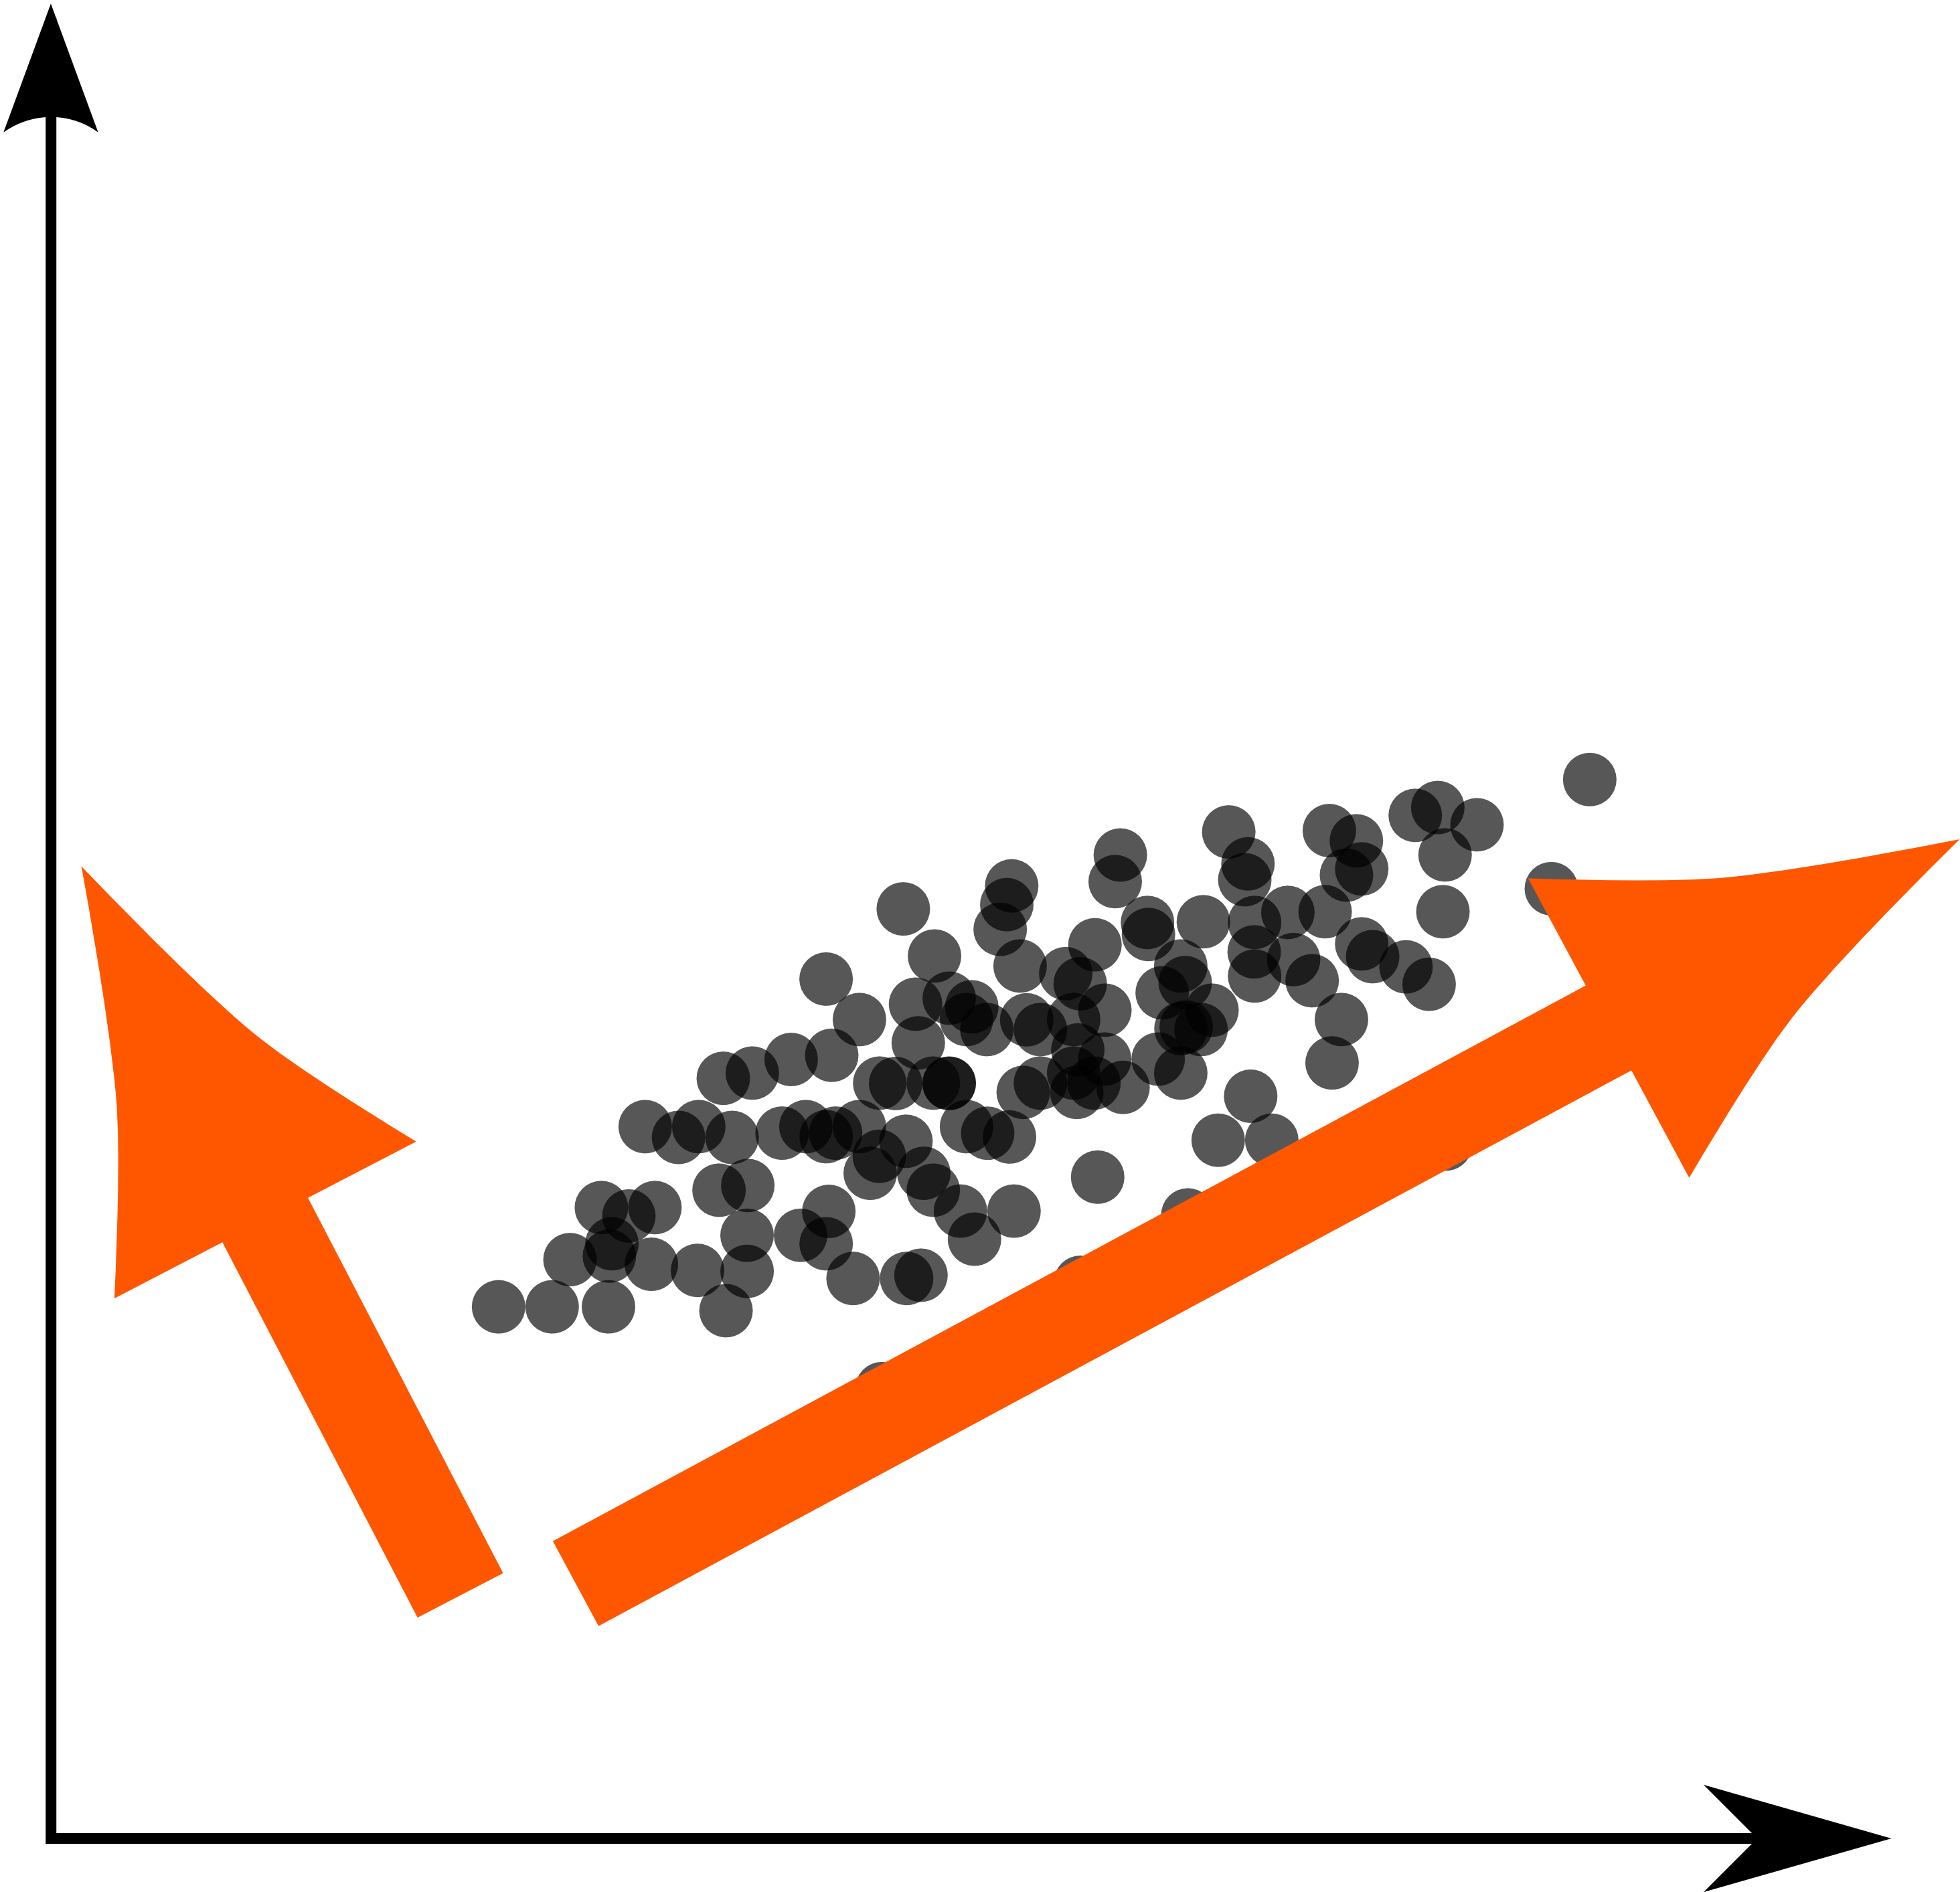
\includegraphics[scale=.5]{svg/qrimg}
    } &  
    \only<2->{
       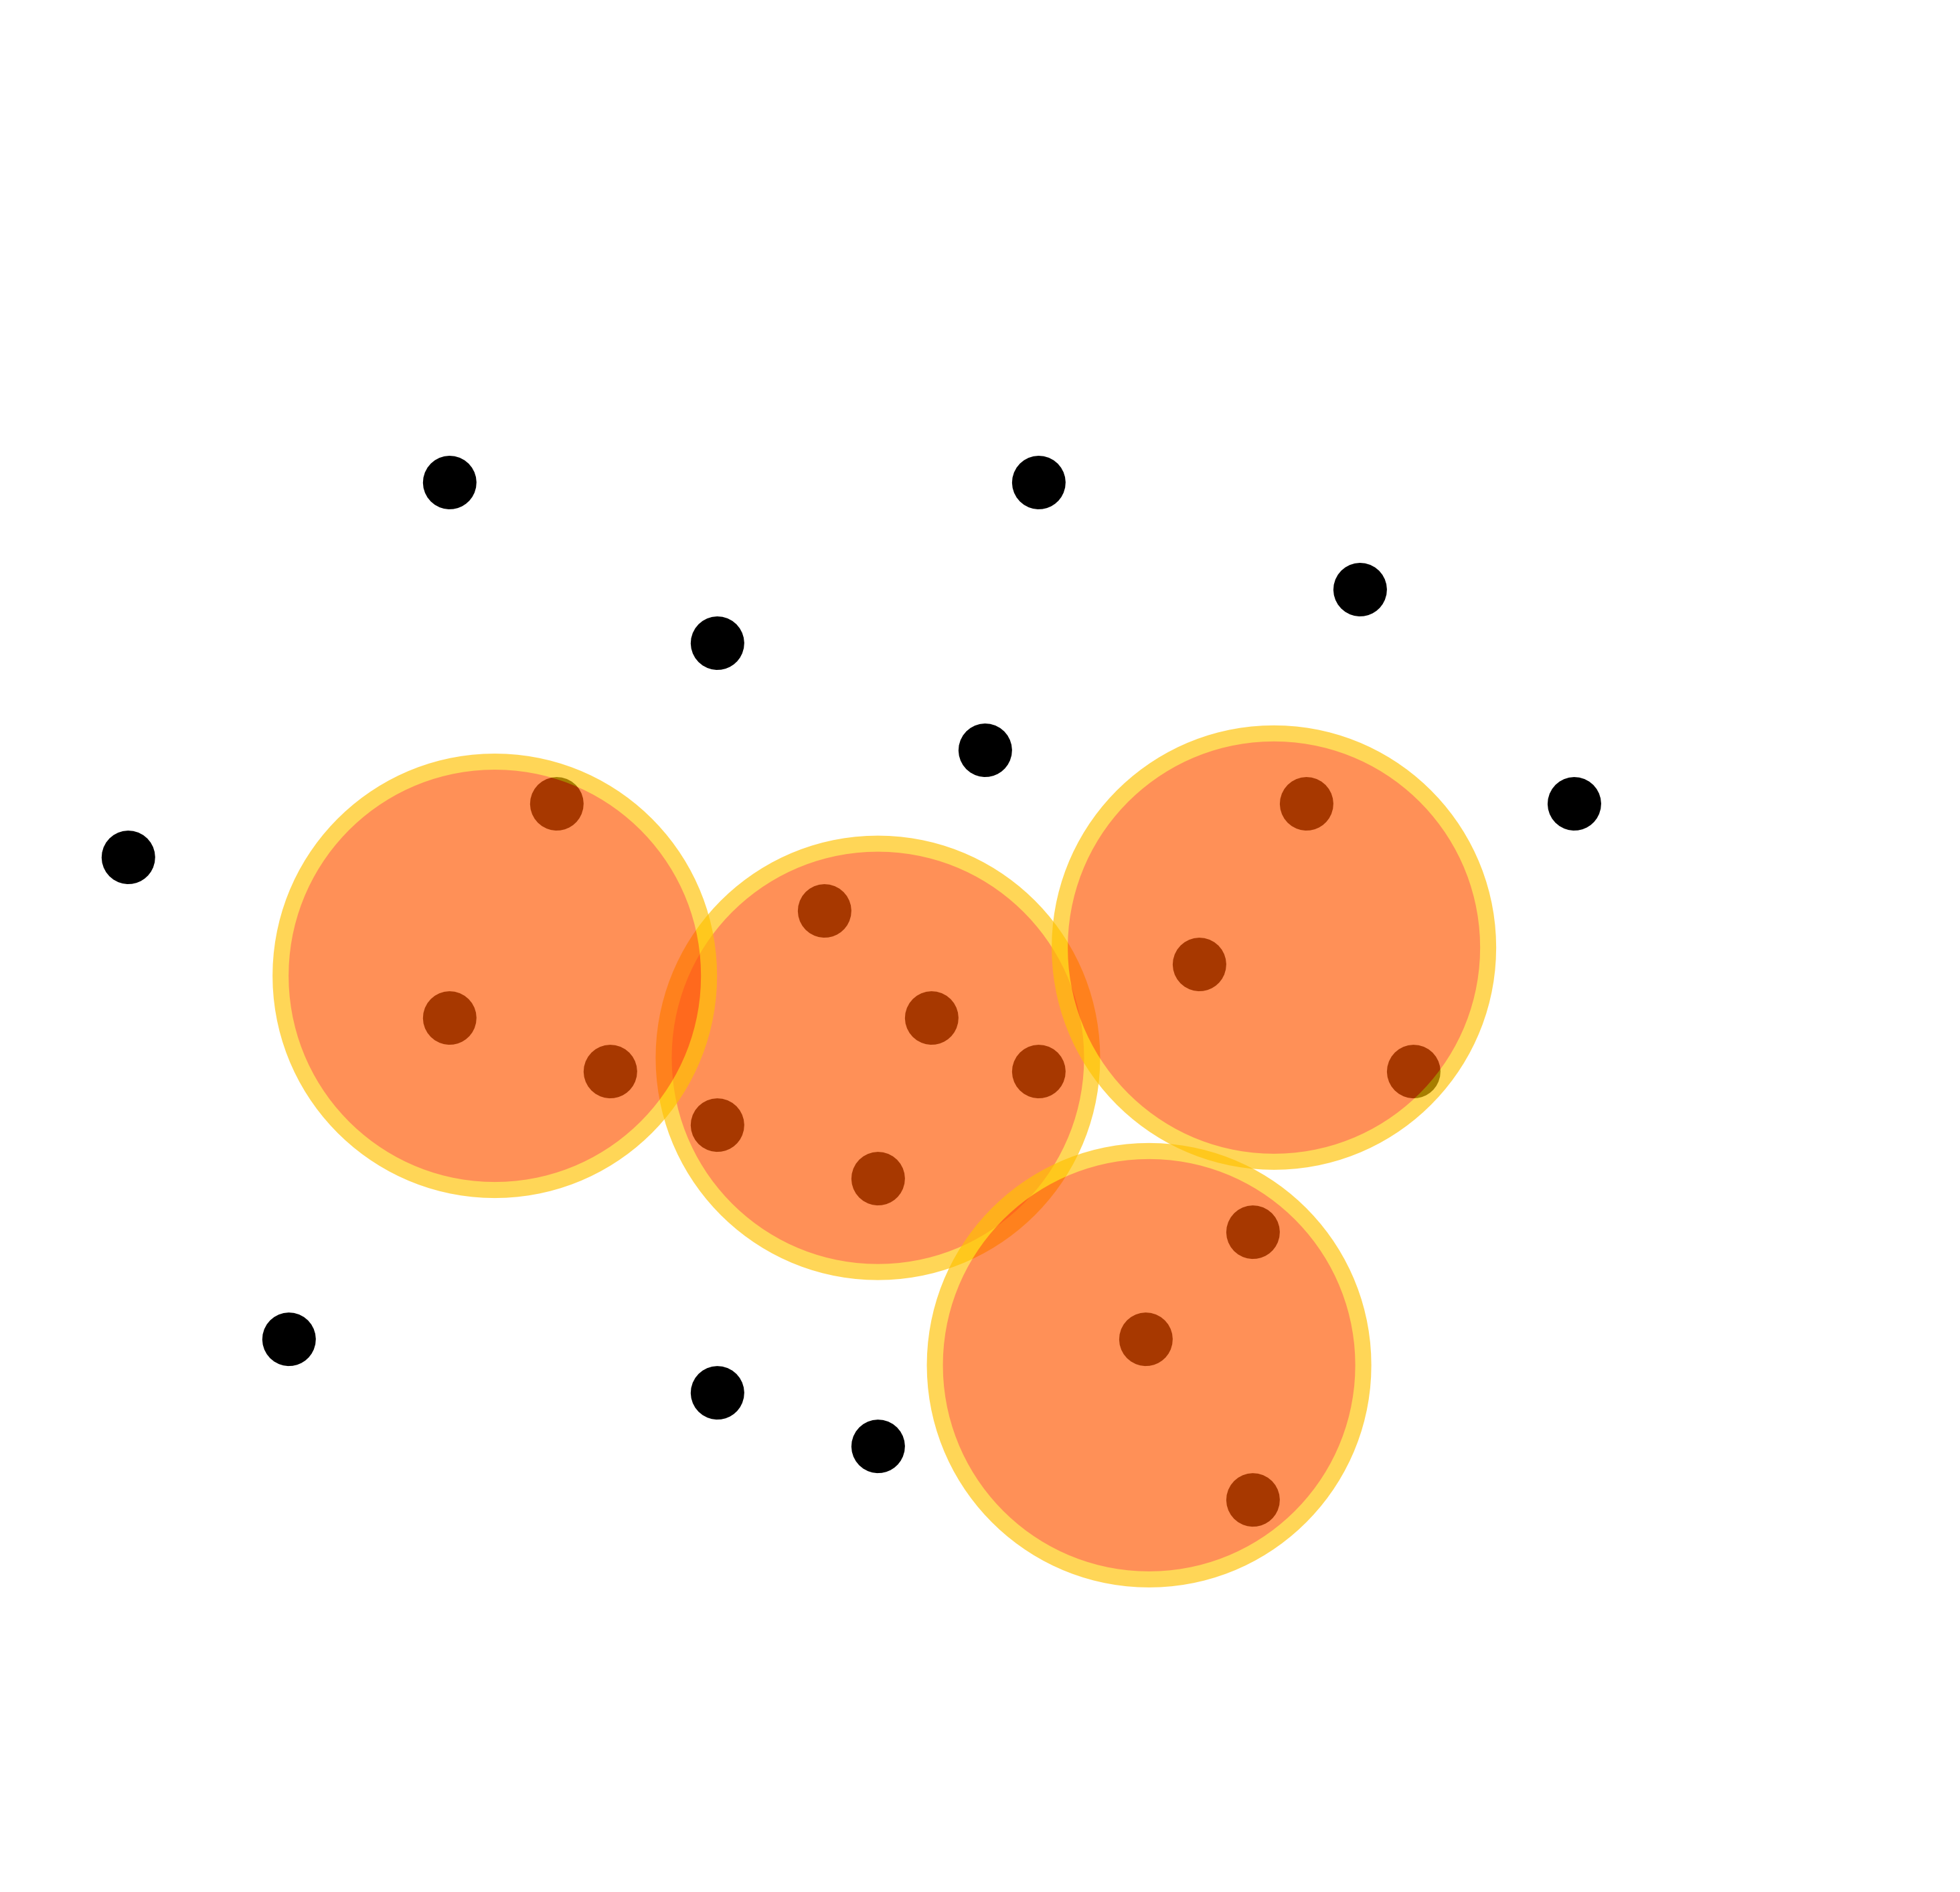
\includegraphics[scale=.5]{svg/ilpimg}
   } &
    \only<3->{
       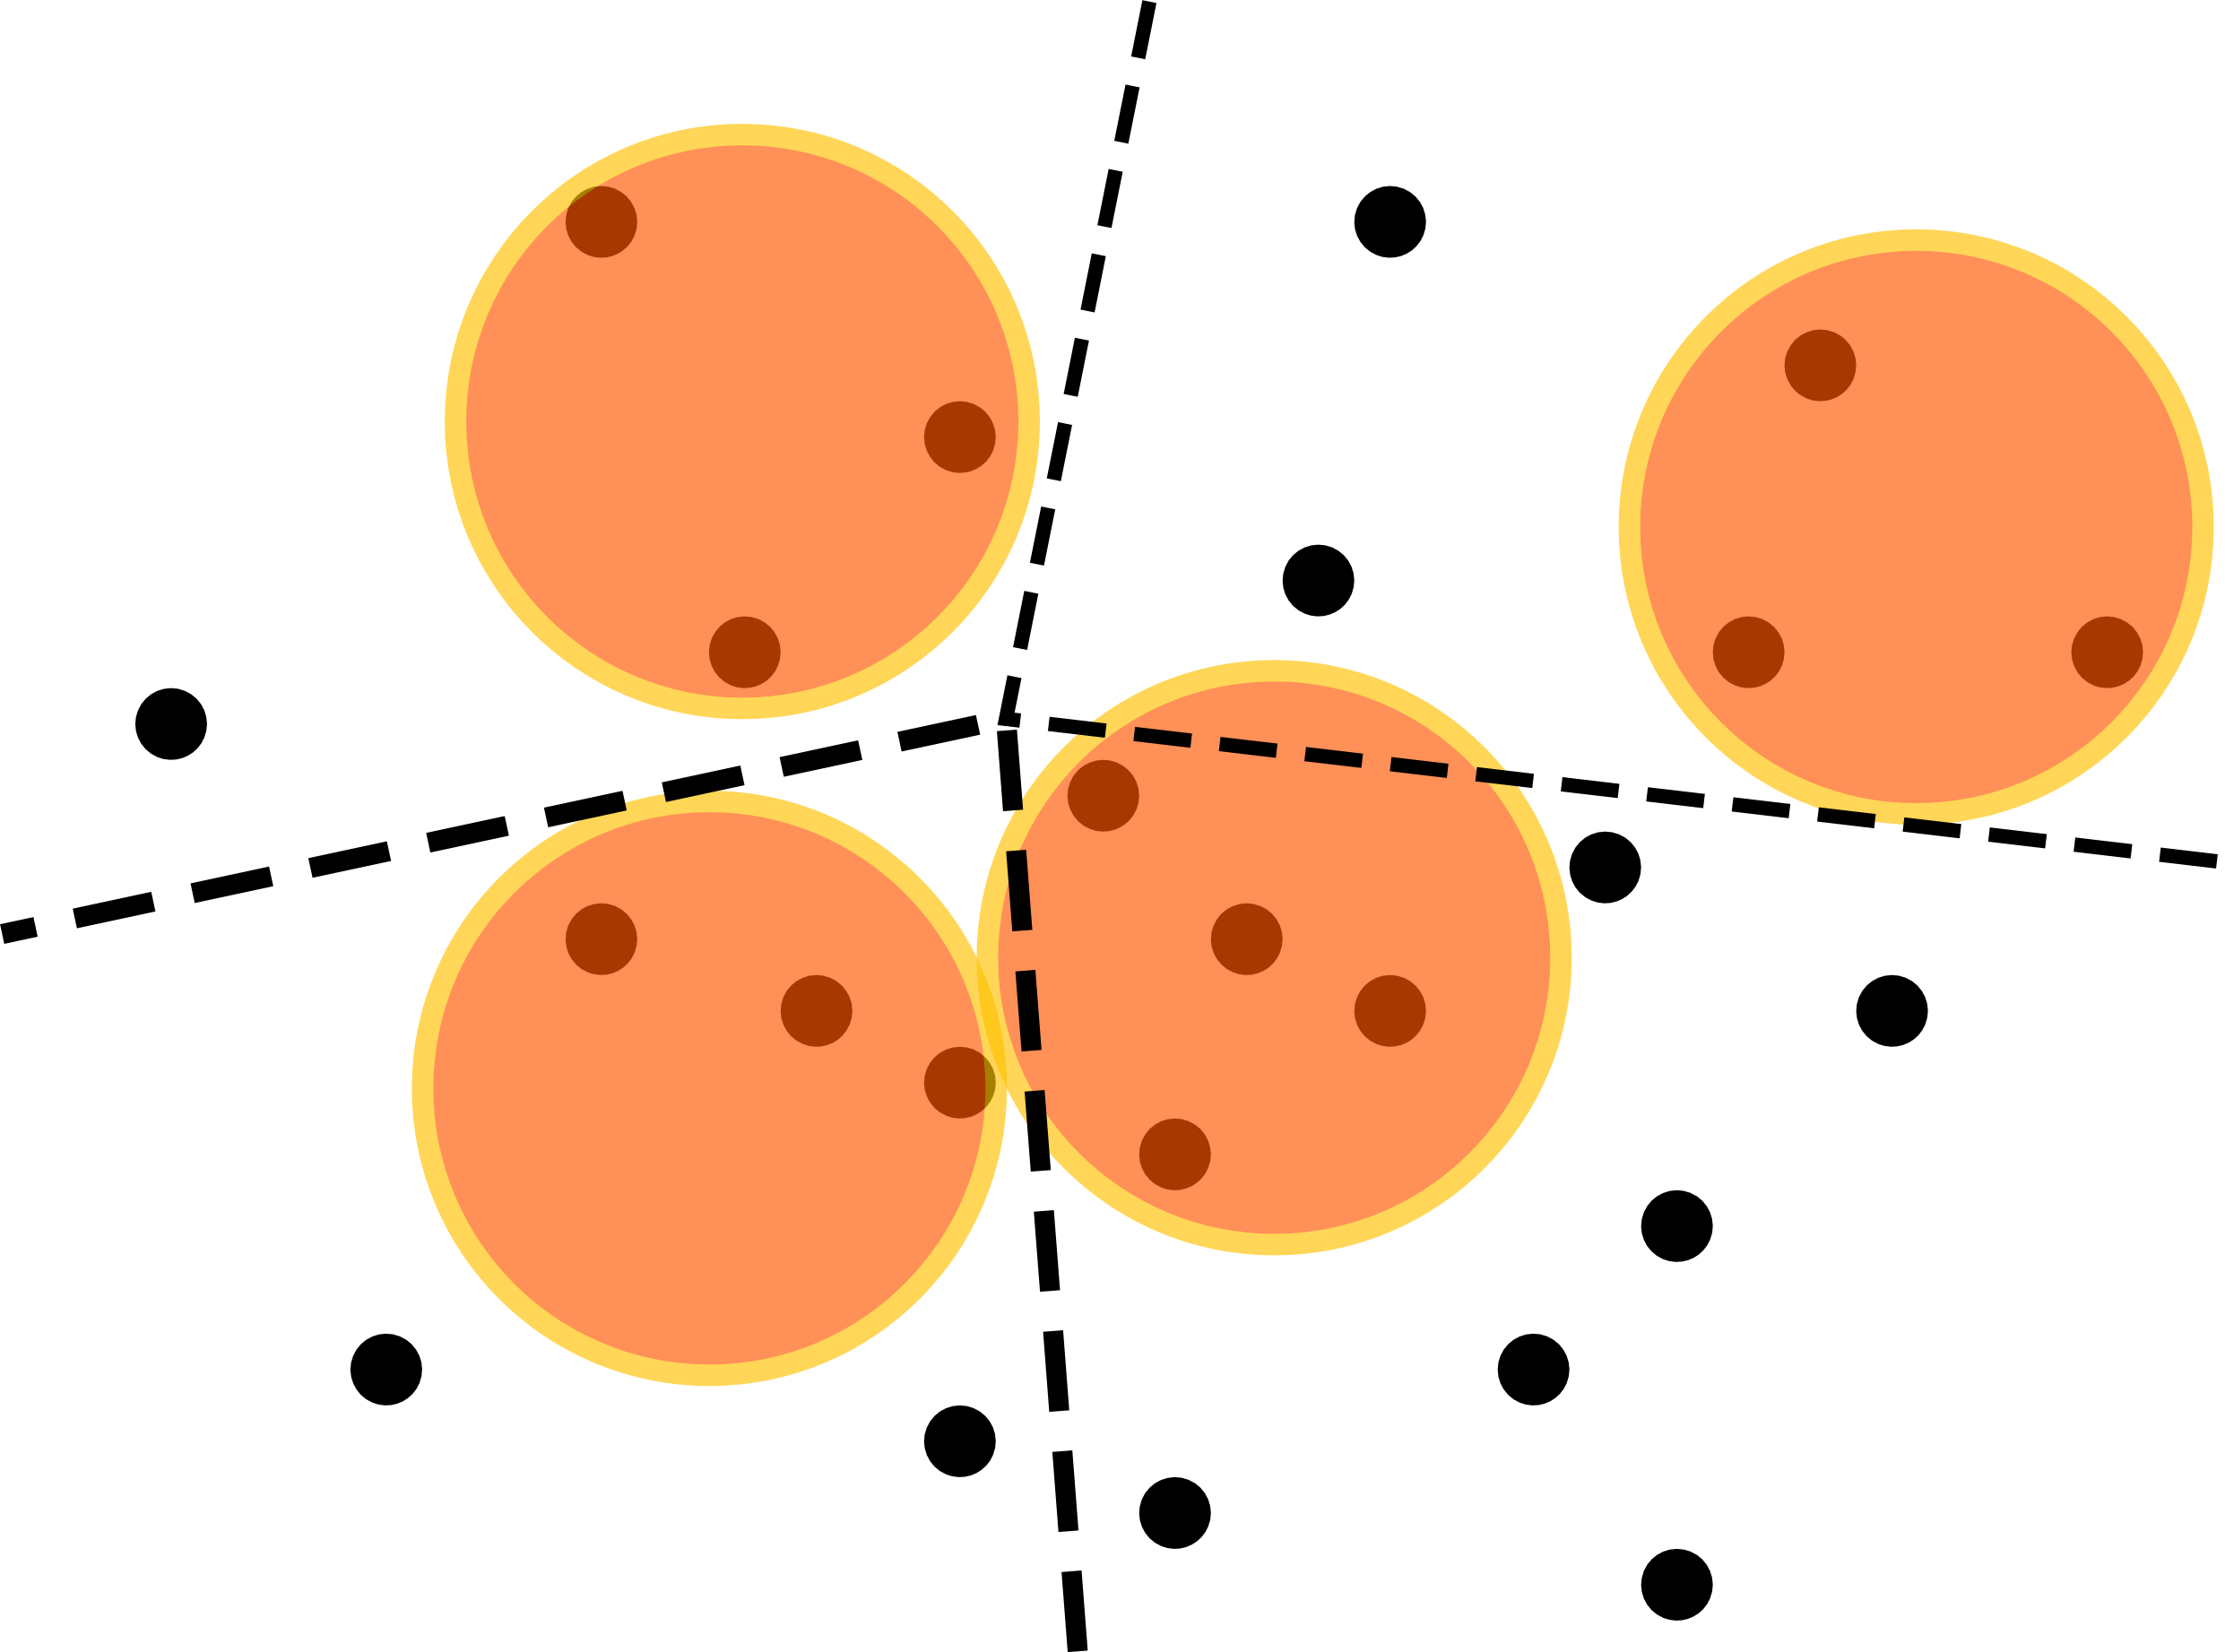
\includegraphics[scale=.5]{svg/smimg}
    } \\
    \uncover<1->{QR decomp.} &\uncover<2->{ILP} & \uncover<3>{Submodular} \\
\end{tabular}
  \end{itemize}


\end{frame}


\begin{frame}{Extraction by Optimization}
    \begin{itemize}
   \only<1>{\item All are components of 
            state-of-the-art extractive newswire summarization systems
        \citep{hong2014repository}.}
   \only<2->{\proit{All are components of 
            state-of-the-art extractive newswire summarization systems
            \citep{hong2014repository}.}}

   \only<-2>{\item ILP formulations very flexible with constraint handling.}
   \only<3->{\proit{ILP formulations very flexible with constraint 
       handling.}}
   \only<-3>{\item ILP possibly less scalable than QR decomposition or 
       submodular optimization.}
   \only<4->{\conit{ILP possibly less scalable than QR 
           decomposition or submodular optimization.}}
   \only<-4>{\item \citep{gillick2009global} ILP matched oracle level ROUGE 
                scores;\\
        optimization based extractive summarization may be at the 
        upper limit of ROUGE scores.}
   \only<5->{\proit{\citep{gillick2009global} ILP matched oracle
               level ROUGE  scores;\\
        optimization based extractive summarizers may be at the 
        upper limit of ROUGE scores.}}
    \end{itemize}
\end{frame}

\begin{frame}{Extractive Summarization}

 \begin{itemize}
  \item Extractive summarization has focused mostly on maximizing content
    selection scores (ROUGE and Pyramid).
~\\
~\\
  \item Global optimization of coverage correlates with shallow coverage 
        metrics.
~\\
~\\
  \item Perhaps we have reached the limit of extractive summarization? 
 \end{itemize}

\end{frame}

\section{Abstraction}


%%\begin{frame}{Abstraction Paradigms}
%%    \begin{itemize}
%%        \item \textbf{Sentence Fusion} combine several similar sentences into
%%            one sentence
%%        \item \textbf{Compression} selectively remove words/phrases that 
%%            are less important 
%%    \end{itemize}
%%\end{frame}
%
\begin{frame}[t]{
    \only<1-3>{Abstractive Summarization}\only<4->{Fusion}}
  \begin{figure}[h]
    \centering
    \begin{tikzpicture}
   
        \visible<1-3>{
        \node at (0,0) {
\includegraphics[scale=.1]{fusion_icon}};
        \node at (0,-.5) {\tiny \cite{barzilay2005sentence}};
        \node at (0,-1.1) {
\includegraphics[scale=.1]{fusion_icon}};
        \node at (0,-1.6) {\tiny \cite{filippova2008sentence}};
        }

        \visible<2-3>{\node at (0,-5.2) {\Large \textbf{Fusion}};}
        \visible<4->{\node at (0,-5.2) 
            {\Large\textcolor{proc}{\textbf{Fusion}}};}
        \visible<4->{
        \node at (0,0) {
\includegraphics[scale=.12]{fusion_icon}};
        \node at (0,-.5) 
            {\tiny \textcolor{proc}{\cite{barzilay2005sentence}}};
        \node at (0,-1.1) {
\includegraphics[scale=.12]{fusion_icon}};
        \node at (0,-1.6) 
            {\tiny \textcolor{proc}{\cite{filippova2008sentence}}};
        }

        \node at (3.25,1.5) {\includegraphics[scale=.07]{compression_icon}};
        \node at (2.95,1.6) {\includegraphics[scale=.09]{extract_icon}};
        \node at (3.25,1) {\tiny \cite{zajic2006sentence}};
        \node at (3.25,0) {\includegraphics[scale=.07]{compression_icon}};
        \node at (2.95,.1) {\includegraphics[scale=.09]{extract_icon}};
        \node at (3.25,-.5) {\tiny \cite{martins2009summarization}};
        \node at (3.25,-1.1) {\includegraphics[scale=.07]{compression_icon}};
        \node at (2.95,-1) {\includegraphics[scale=.09]{extract_icon}};
        \node at (3.25,-1.6) {\tiny \cite{berg2011jointly}};
        \node at (3.25,-2.6) {\includegraphics[scale=.07]{compression_icon}};
        \node at (2.95,-2.5) {\includegraphics[scale=.09]{extract_icon}};
        \node at (3.25,-3.1) {\tiny \cite{wang2013sentence}};
        
        \visible<3->{\node at (3.25,-4.5) {\textbf{Extraction}};}

        \node at (6.25,1) {\includegraphics[scale=.07]{compression_icon}};
        \node at (5.95,1.2) {\includegraphics[scale=.06]{align_icon}};
        \node at (6.25,.5) {\tiny \cite{woodsend2010generation}};
        \node at (6.25,-.1) {\includegraphics[scale=.07]{compression_icon}};
        \node at (5.95,.1) {\includegraphics[scale=.06]{align_icon}};
        \node at (6.25,-.6) {\tiny \cite{rush2015neural}};

        \visible<3->{\draw[thick,dotted] (4.8,-4) edge (4.8,2);} 

        \node at (5.75,-1.9) {\includegraphics[scale=.11]{amr_icon}};
        \node at (6.25,-2.0) {\includegraphics[scale=.07]{compression_icon}};
        \node at (6.25,-2.5) {\tiny \cite{pighin2014modelling}};
        \node at (5.75,-3) {\includegraphics[scale=.11]{amr_icon}};
        \node at (6.25,-3.1) {\includegraphics[scale=.07]{compression_icon}};
        \node at (6.25,-3.6) {\tiny \cite{liu2015toward}};
        \visible<3->{\node at (6.25,-4.5) {\textbf{Generation}};}
        \visible<2>{\node at (4.75,-5.2 ) {\Large \textbf{Compression}};}
        \visible<3->{\node at (4.75,-5.2 ) {\Large \textbf{+Compression}};}
        \visible<2-3>{
            \draw[thick,dotted] (-1.5,2) rectangle (1.5,-5.5);
            \draw[thick,dotted] (1.74,2) rectangle (7.5,-5.5);}
        \visible<4->{
            \draw[thick,dotted] (1.74,2) rectangle (7.5,-5.5);
            \draw[thick,dotted,draw=proc] (-1.5,2) rectangle (1.5,-5.5);
        }

    \end{tikzpicture}
  \end{figure}
\end{frame}

\begin{frame}{Fusion in MDS} 
    \begin{enumerate}
        \item Content Aggregation, \\
            (theme selection in \cite{barzilay2005sentence}), \\
            i.e. cluster input sentences.
        \item Order clusters.
        \item Fuse clusters.
    \end{enumerate}
\end{frame}

\begin{frame}[t]{Sentence Fusion}
    \large{\textbf{\cite{barzilay2005sentence}}} 
    \begin{itemize}
        \small
        \item Align dependency graphs; form fusion lattice.
        \item Linearize lattice with a language model.
        \only<1>{\item Output has low content coverage vs. human.}
        \only<2->{\conit{Output has low content coverage vs. human.}}
        \only<-2>{\item Linearization is the source of grammatical errors.}
        \only<3->{\conit{Linearization is the source of grammatical errors.}}
    \end{itemize}
       
 \only<-3>{
  \begin{figure}[h]
   \centering
   \includegraphics[scale=.25,angle=90]{fusion-lattice} 
  \end{figure}
~\\
 }
 \only<4->{
  {\large\textbf{\cite{filippova2008sentence}}} \\
  \begin{itemize}
   \small
   \item Compress aligned dependency graph using ILP formulation.
   \item Deletion conditioned on informativeness and attachment
        scores.
   \only<-4>{\item Better readability scores than 
        {\small\citep{barzilay2005sentence}}.}
   \only<5->{\proit{Better readability scores than 
       {\small\citep{barzilay2005sentence}}}.}
  \end{itemize}

  \begin{itemize}
   \small
   \only<-5>{\item[]  Both system evaluated on small/non-standard datasets.}
   \only<6->{\conit{Both system evaluated on small/non-standard datasets.}}
   \only<-6>{\item[] Hard to say how comparable to competitive extractive 
    system.}
   \only<7->{\conit{Hard to say how comparable to competitive extractive 
    system.}}
  \end{itemize}
 }
\end{frame}

\begin{frame}[t]{
    \only<1>{Fusion}\only<2>{Abstractive Summarization}\only<3>{Compression and Extraction}}
  \begin{figure}[h]
    \centering
    \begin{tikzpicture}
   
        \visible<1>{
        \node at (0,0) {\includegraphics[scale=.12]{fusion_icon}};
        \node at (0,-.5) 
            {\tiny \textcolor{proc}{\cite{barzilay2005sentence}}};
        \node at (0,-1.1) {\includegraphics[scale=.12]{fusion_icon}};
        \node at (0,-1.6) 
            {\tiny \textcolor{proc}{\cite{filippova2008sentence}}};

        \node at (0,-5.2) {\Large \textcolor{proc}{\textbf{Fusion}}};
        \draw[thick,dotted,draw=proc] (-1.5,2) rectangle (1.5,-5.5);
        }

        \visible<2->{
        \node at (0,0) {\includegraphics[scale=.1]{fusion_icon}};
        \node at (0,-.5) {\tiny \cite{barzilay2005sentence}};
        \node at (0,-1.1) {\includegraphics[scale=.1]{fusion_icon}};
        \node at (0,-1.6) {\tiny \cite{filippova2008sentence}};

        \node at (0,-5.2) {\Large \textbf{Fusion}};
        \draw[thick,dotted] (-1.5,2) rectangle (1.5,-5.5);
        }

        \visible<-2>{
        \node at (3.25,1.5) {\includegraphics[scale=.07]{compression_icon}};
        \node at (2.95,1.6) {\includegraphics[scale=.09]{extract_icon}};
        \node at (3.25,1) {\tiny \cite{zajic2006sentence}};
        \node at (3.25,0) {\includegraphics[scale=.07]{compression_icon}};
        \node at (2.95,.1) {\includegraphics[scale=.09]{extract_icon}};
        \node at (3.25,-.5) {\tiny \cite{martins2009summarization}};
        \node at (3.25,-1.1) {\includegraphics[scale=.07]{compression_icon}};
        \node at (2.95,-1) {\includegraphics[scale=.09]{extract_icon}};
        \node at (3.25,-1.6) {\tiny \cite{berg2011jointly}};
        \node at (3.25,-2.6) {\includegraphics[scale=.07]{compression_icon}};
        \node at (2.95,-2.5) {\includegraphics[scale=.09]{extract_icon}};
        \node at (3.25,-3.1) {\tiny \cite{wang2013sentence}};
        
        \node at (3.25,-4.5) {\textbf{Extraction}};
        \draw[thick,dotted] (4.8,-4) edge (4.8,2); 
        \draw[thick,dotted] (1.74,2) rectangle (7.5,-5.5);
        \node at (4.75,-5.2 ) {\Large \textbf{+Compression}};
        }

        \visible<3>{
        \node at (3.25,1.5) {\includegraphics[scale=.09]{compression_icon}};
        \node at (2.95,1.6) {\includegraphics[scale=.11]{extract_icon}};
        \node at (3.25,1) {\tiny \textcolor{proc}{\cite{zajic2006sentence}}};
        \node at (3.25,0) {\includegraphics[scale=.09]{compression_icon}};
        \node at (2.95,.1) {\includegraphics[scale=.11]{extract_icon}};
        \node at (3.25,-.5) {\tiny \textcolor{proc}{\cite{martins2009summarization}}};
        \node at (3.25,-1.1) {\includegraphics[scale=.09]{compression_icon}};
        \node at (2.95,-1) {\includegraphics[scale=.11]{extract_icon}};
        \node at (3.25,-1.6) {\tiny \textcolor{proc}{\cite{berg2011jointly}}};
        \node at (3.25,-2.6) {\includegraphics[scale=.09]{compression_icon}};
        \node at (2.95,-2.5) {\includegraphics[scale=.11]{extract_icon}};
        \node at (3.25,-3.1) {\tiny \textcolor{proc}{\cite{wang2013sentence}}};
        
        \node at (3.25,-4.5) {\textcolor{proc}{\textbf{Extraction}}};
        \draw[thick,dotted,draw=proc] (4.8,-4) edge (4.8,2); 
        \draw[thick,dotted,draw=proc] (1.74,2) rectangle (7.5,-5.5);
        \node at (4.75,-5.2 ) {\Large \textcolor{proc}{\textbf{+Compression}}};
        }

        \node at (6.25,1) {\includegraphics[scale=.07]{compression_icon}};
        \node at (5.95,1.2) {\includegraphics[scale=.06]{align_icon}};
        \node at (6.25,.5) {\tiny \cite{woodsend2010generation}};
        \node at (6.25,-.1) {\includegraphics[scale=.07]{compression_icon}};
        \node at (5.95,.1) {\includegraphics[scale=.06]{align_icon}};
        \node at (6.25,-.6) {\tiny \cite{rush2015neural}};


        \node at (5.75,-1.9) {\includegraphics[scale=.11]{amr_icon}};
        \node at (6.25,-2.0) {\includegraphics[scale=.07]{compression_icon}};
        \node at (6.25,-2.5) {\tiny \cite{pighin2014modelling}};
        \node at (5.75,-3) {\includegraphics[scale=.11]{amr_icon}};
        \node at (6.25,-3.1) {\includegraphics[scale=.07]{compression_icon}};
        \node at (6.25,-3.6) {\tiny \cite{liu2015toward}};
        \node at (6.25,-4.5) {\textbf{Generation}};

    \end{tikzpicture}
  \end{figure}
\end{frame}


%\begin{frame}{Compression with Extraction} 
%
%  \only<1>{
%    Extract sentences while selectively deleting less important words/phrases
%    from the input.
%  }
%    
%  \only<2>{
%    \textbf{Extract} sentences while selectively deleting less important 
%    words/phrases from the input.
%  }
%
%  \only<3>{
%    \textbf{Extract} sentences while selectively \textbf{deleting} less 
%    important words/phrases from the input.
%  }
%
%\end{frame}

\begin{frame}{Compression with Extraction: Heuristic Pruning} 
  \textbf{\cite{zajic2006sentence} }
  \begin{enumerate}
    \small
    \item Over generate sentence compressions \\
        \spit (linguistically informed heuristics).
    \item Perform extractive ranking based summarization.
  \end{enumerate}
  \uncover<2->{
    \begin{itemize}
        \small
        \only<-2>{\item Manually tuned ranking weights.}
        \only<3->{\conit{Manually tuned ranking weights.}}
        \only<-3>{\item Moderate to poor ROUGE results.}
        \only<4->{\conit{Moderate to poor ROUGE results.}}
        \only<-4>{\item Poor linguistic quality judgements.}
        \only<5->{\conit{Poor linguistic quality judgements.}}
    \end{itemize}
  }
\end{frame}


\begin{frame}{Compression with Extraction: ILP}
  \textbf{\cite{martins2009summarization} }
    \begin{itemize}
      \item Extraction and compression task is encoded as an ILP.
      \item Extraction \& compression parameters trained separately.
      \only<1>{\item ROUGE-2 scores equivalent to extractive baselines.}
      \only<2->{\conit{ROUGE-2 scores equivalent to extractive baselines.}}
    \end{itemize}

    \textbf{\cite{berg2011jointly} }
    \begin{itemize}
      \only<-2>{\item learn compression and extraction simultaneously (also 
        ILP).}
      \only<3->{\proit{learn compression and extraction simultaneously (also 
        ILP).}}
      \item Used Mechanical Turk to collect labeled data for joint task.
      \only<-3>{\item In practice, uses approximation of joint objective: }
      \only<4>{\conit{In practice, uses approximation of joint objective: }}
        \begin{enumerate}
            \item Run overlength extractive solver.
            \item Run compressive solver over fixed extractions.
        \end{enumerate}
      \end{itemize}
\end{frame}



\begin{frame}{Compression in with Extraction: Beam Search} 
    \textbf{\cite{wang2013sentence}}
    \begin{enumerate}
        \small
        \item Rank \& Order sentences.
        \item Compress sentences.
        \item Add sentences to summary until length limit reached.
    \end{enumerate}
    \uncover<2->{
      \begin{itemize}
        \small
        \item Ranking and compression trained separately.
        \only<-2>{\item Ranking performed on uncompressed sentences.}
        \only<3->{\conit{Ranking performed on uncompressed sentences.}}
        \item Linguistically motivated beam search is used to find 
            approximate best compressions.
        \only<-3>{\item Beats extractive systems on query focused 
            summarization in ROUGE-2/Pyramid.}
        \only<4->{\proit{Beats extractive systems on query focused 
            summarization in ROUGE-2/Pyramid.}}
        \only<-4>{\item Comparable to extractive systems w.r.t. linguistic 
            quality.}
        \only<5->{\proit{Comparable to extractive systems w.r.t. linguistic
            quality.}}
    \end{itemize}
}
\end{frame}

\begin{frame}{
    \only<1>{Compression and Extraction}\only<2>{Abstractive Summarization}\only<3>{Compression and Generation}}
  \begin{figure}[h]
    \centering
    \begin{tikzpicture}
    
        \node at (0,0) {\includegraphics[scale=.1]{fusion_icon}};
        \node at (0,-.5) {\tiny \cite{barzilay2005sentence}};
        \node at (0,-1.1) {\includegraphics[scale=.1]{fusion_icon}};
        \node at (0,-1.6) {\tiny \cite{filippova2008sentence}};

        \node at (0,-5.2) {\Large \textbf{Fusion}};
        \draw[thick,dotted] (-1.5,2) rectangle (1.5,-5.5);

        \visible<1>{
        \node at (3.25,1.5) {\includegraphics[scale=.09]{compression_icon}};
        \node at (2.95,1.6) {\includegraphics[scale=.11]{extract_icon}};
        \node at (3.25,1) {\tiny \textcolor{proc}{\cite{zajic2006sentence}}};
        \node at (3.25,0) {\includegraphics[scale=.09]{compression_icon}};
        \node at (2.95,.1) {\includegraphics[scale=.11]{extract_icon}};
        \node at (3.25,-.5) {\tiny \textcolor{proc}{\cite{martins2009summarization}}};
        \node at (3.25,-1.1) {\includegraphics[scale=.09]{compression_icon}};
        \node at (2.95,-1) {\includegraphics[scale=.11]{extract_icon}};
        \node at (3.25,-1.6) {\tiny \textcolor{proc}{\cite{berg2011jointly}}};
        \node at (3.25,-2.6) {\includegraphics[scale=.09]{compression_icon}};
        \node at (2.95,-2.5) {\includegraphics[scale=.11]{extract_icon}};
        \node at (3.25,-3.1) {\tiny \textcolor{proc}{\cite{wang2013sentence}}};
        
        \node at (3.25,-4.5) {\textcolor{proc}{\textbf{Extraction}}};
        \draw[thick,dotted,draw=proc] (4.8,-4) edge (4.8,2); 
        \draw[thick,dotted,draw=proc] (1.74,2) rectangle (7.5,-5.5);
        \node at (4.75,-5.2 ) {\Large \textcolor{proc}{\textbf{+Compression}}};
        }

        \visible<2->{
        \node at (3.25,1.5) {\includegraphics[scale=.07]{compression_icon}};
        \node at (2.95,1.6) {\includegraphics[scale=.09]{extract_icon}};
        \node at (3.25,1) {\tiny \cite{zajic2006sentence}};
        \node at (3.25,0) {\includegraphics[scale=.07]{compression_icon}};
        \node at (2.95,.1) {\includegraphics[scale=.09]{extract_icon}};
        \node at (3.25,-.5) {\tiny \cite{martins2009summarization}};
        \node at (3.25,-1.1) {\includegraphics[scale=.07]{compression_icon}};
        \node at (2.95,-1) {\includegraphics[scale=.09]{extract_icon}};
        \node at (3.25,-1.6) {\tiny \cite{berg2011jointly}};
        \node at (3.25,-2.6) {\includegraphics[scale=.07]{compression_icon}};
        \node at (2.95,-2.5) {\includegraphics[scale=.09]{extract_icon}};
        \node at (3.25,-3.1) {\tiny \cite{wang2013sentence}};
        
        \node at (3.25,-4.5) {\textbf{Extraction}};
        \draw[thick,dotted] (4.8,-4) edge (4.8,2); 
        \draw[thick,dotted] (1.74,2) rectangle (7.5,-5.5);
        \node at (4.75,-5.2 ) {\Large \textbf{+Compression}};
        }




        \visible<-2>{
        \node at (6.25,1) {\includegraphics[scale=.07]{compression_icon}};
        \node at (5.95,1.2) {\includegraphics[scale=.06]{align_icon}};
        \node at (6.25,.5) {\tiny \cite{woodsend2010generation}};
        \node at (6.25,-.1) {\includegraphics[scale=.07]{compression_icon}};
        \node at (5.95,.1) {\includegraphics[scale=.06]{align_icon}};
        \node at (6.25,-.6) {\tiny \cite{rush2015neural}};

        \node at (5.75,-1.9) {\includegraphics[scale=.11]{amr_icon}};
        \node at (6.25,-2.0) {\includegraphics[scale=.07]{compression_icon}};
        \node at (6.25,-2.5) {\tiny \cite{pighin2014modelling}};
        \node at (5.75,-3) {\includegraphics[scale=.11]{amr_icon}};
        \node at (6.25,-3.1) {\includegraphics[scale=.07]{compression_icon}};
        \node at (6.25,-3.6) {\tiny \cite{liu2015toward}};
        \node at (6.25,-4.5) {\textbf{Generation}};
        }

        \visible<3>{
        \node at (6.25,1) {\includegraphics[scale=.07]{compression_icon}};
        \node at (5.95,1.2) {\includegraphics[scale=.06]{align_icon}};
        \node at (6.25,.5) {\tiny \textcolor{proc}{\cite{woodsend2010generation}}};
        \node at (6.25,-.1) {\includegraphics[scale=.07]{compression_icon}};
        \node at (5.95,.1) {\includegraphics[scale=.06]{align_icon}};
        \node at (6.25,-.6) {\tiny \textcolor{proc}{\cite{rush2015neural}}};

        \node at (5.75,-1.9) {\includegraphics[scale=.11]{amr_icon}};
        \node at (6.25,-2.0) {\includegraphics[scale=.07]{compression_icon}};
        \node at (6.25,-2.5) {\tiny \textcolor{proc}{\cite{pighin2014modelling}}};
        \node at (5.75,-3) {\includegraphics[scale=.11]{amr_icon}};
        \node at (6.25,-3.1) {\includegraphics[scale=.07]{compression_icon}};
        \node at (6.25,-3.6) {\tiny \textcolor{proc}{\cite{liu2015toward}}};
        \node at (6.25,-4.5) {\textcolor{proc}{\textbf{Generation}}};
        \node at (4.75,-5.2 ) {\Large \textcolor{proc}{\textbf{+Compression}}};
        \draw[thick,dotted,draw=proc] (4.8,-4) edge (4.8,2); 
        \draw[thick,dotted,draw=proc] (1.74,2) rectangle (7.5,-5.5);
        }


    \end{tikzpicture}
  \end{figure}
\end{frame}

\begin{frame}{Compressive Generation}

    \only<1>{\textbf{Alignments}}
    \only<2->{\textcolor{proc}{\textbf{Alignments}}}
    \begin{itemize}
      \item \textbf{Quasi-Synchronous Grammar} 
       {\scriptsize \citep{woodsend2010generation}}
      \item \textbf{Attentional Neural MT}
       {\scriptsize \citep{rush2015neural}}
    \end{itemize}

    \textbf{Semantics}
    \begin{itemize}
      \item \textbf{Open Information Extraction} 
       {\scriptsize \citep{pighin2014modelling}}
      \item \textbf{Abstract Meaning Representation} 
       {\scriptsize \citep{liu2015toward}}
    \end{itemize}
\end{frame}
    
    
\begin{frame}{Compressive Alignments}

 \large{\textbf{\cite{woodsend2010generation}}} -- Generation as parsing.
 \begin{itemize}
   \small
   \item Find compressive derivation of input under quasi-synchronous 
        grammar. 
   \item Similar to ILP's for compression/extraction, but 
   \only<1>{more expressive}\only<2->{\textcolor{proc}{more expressive}}:
   \begin{itemize}
     \item deletion (compression)
     \item rewriting (paraphrase)
     \item reordering 
   \end{itemize}
   \only<-2>{\item High grammaticality and importance scores\\
       \spit (on par with human reference).
   }
   \only<3->{\proit{High grammaticality and importance scores \\
       \spit (on par with human reference).
    }}
 \end{itemize}

 \only<-3>{
    \begin{figure}[h]
        \centering
        \includegraphics[scale=.22]{backup/images/figure2-woodsend10}
    \end{figure}
 }

 \only<4->{
 \large{\textbf{\cite{rush2015neural}}} -- Generation as machine translation.
 \begin{itemize}
   \small
   \item Finds soft alignments between input and compressive generation.
   \only<-4>{\item Both neural attention 
            model and MOSES are state-of-the-art w.r.t. ROUGE-2.}
   \only<5->{\proit{Both neural attention 
   model and MOSES are state-of-the-art w.r.t. ROUGE-2.}}
   \only<-5>{\item Discrete features needed to surpass MOSES.}
   \only<6->{\proit{Discrete features needed to surpass MOSES.}}
 \end{itemize}
 }
\end{frame}

\begin{frame}{Compressive Generation}

    \only<1>{\textcolor{proc}{\textbf{Alignments}}}
    \only<2->{\textbf{Alignments}}
    \begin{itemize}
      \item \textbf{Quasi-Synchronous Grammar} 
       {\scriptsize \citep{woodsend2010generation}}
      \item \textbf{Attentional Neural MT}
       {\scriptsize \citep{rush2015neural}}
    \end{itemize}

    \only<-2>{\textbf{Semantics}}
    \only<3>{\textcolor{proc}{\textbf{Semantics}}}
    \begin{itemize}
      \item \textbf{Open Information Extraction} 
       {\scriptsize \citep{pighin2014modelling}}
      \item \textbf{Abstract Meaning Representation} 
       {\scriptsize \citep{liu2015toward}}
    \end{itemize}

\end{frame}
 

\begin{frame}{Summarization with Semantics}

 \large{\textbf{\cite{pighin2014modelling}}}
 \begin{itemize}
  \small
  \item Mine template patterns for sentence summarization.
  \item Memory-based look up for probabilistically  mapping a 
        sentence to template.
  \item Only compare against their own template \& compression based methods.\\
  \only<1>{Unclear how these compare to other approaches or human reference.}
  \only<2->{\conit{Unclear how these compare to other approaches or human 
        reference.}}
 \end{itemize}

 \large{\textbf{\cite{liu2015toward}}}
 \begin{enumerate}
  \small
  \item Merge AMR graphs of inputs into a single graph object.
  \item Compress merged graph into valid AMR (using ILP solver).
  \item Generate text from summary AMR (in theory).
 \end{enumerate}
 \begin{itemize}
  \small
  \only<-2>{\item Generation from resultant AMR graph is an open problem.}
  \only<3->{\conit{Generation from resultant AMR graph is an open problem.}}
  \only<-3>{\item Simple unigram generation model used as proof of concept\\
    (large gap between their results and oracle ROUGE-1). }
  \only<4->{\conit{Simple unigram generation model used as proof of concept\\
    (large gap between their results and oracle ROUGE-1).} }
 \end{itemize}
\end{frame}

\begin{frame}{Abstractive Summarization}

  \begin{itemize}
   \only<1>{\item Diverse set of approaches for abstractive generation.}
   \only<2->{\proit{Diverse set of approaches for abstractive generation.}}
~\\
~\\
   \only<-2>{\item Lack of uniform test set makes comparisons difficult:}
   \only<3->{\conit{Lack of uniform test set makes comparisons difficult:}}
   \begin{itemize}
     \item What is the upper bound for content selection?
     \item What is the upper bound for linguistic quality?
   \end{itemize}
~\\
   \only<-3>{\item Lack of automatic linguistic quality evaluation leaves 
    abstractive methods overly focused on ``safe'' deletion rather than 
    writing the best summaries.}
   \only<4>{\conit{Lack of automatic linguistic quality evaluation leaves 
    abstractive methods overly focused on ``safe'' deletion rather than 
    writing the best summaries.}}
 \end{itemize}

\end{frame}


\begin{frame}{Conclusion}
   
    \begin{itemize}
            \small
        \item Evaluation has been too focused on \textbf{content selection}.
        \item \textbf{Global optimization} based methods have reached the limit
            of \textbf{content selection} for \textbf{extractive} 
            summarization.
        
        \item \textbf{Abstractive} summarization is also heavily focused on 
            \textbf{content
            selection} (i.e. using deletion to pack more content into
            the length budget).
    \end{itemize}

    Looking to the future:    
    \begin{itemize}
            \small
     \item More research is needed on interaction of linguistic quality
         and content selection.
        \item More research is needed on human organizational strategies in 
            summarization.
        \item More research is needed on temporal/streaming summarization.
     
        %\item How to humans organize a response to an information need/query?
    \end{itemize}
    \uncover<2>{\textbf{Questions?}}

\end{frame}

%
%
%
%
%
%
%
%
%
%
%
%
%
%%%%%%%%%%%%%%%%%%%%%%%%
%
%%\end{frame}
%%\begin{frame}{Extraction by Coverage Optimization}
%%
%%    \begin{figure}[!h]
%%        \centering
%% \begin{tikzpicture}
%%     \node (C) at (1.5,5) {Classification};
%%     \node[rotate=45] (C) at (4.5,-1.7) {Ranking};
%%     \node[rotate=-45,text=red,opacity=.7] (C) at (-1.5,-1.7) {Coverage Opt.};
%%     \node (C) at (1.5,4) {\includegraphics[scale=.017]{news_icon}};
%%     \node (C) at (1.5,3.7) {\tiny \cite{maskey2005comparing}};
%%     %\node (C) at (1.5,-1) {\includegraphics[scale=.017]{news_icon}};
%%     \node (C) at (0.3,-1.8) {\includegraphics[scale=.022]{news_icon}};
%%     \node[text=red,opacity=.7] (C) at (0.3,-2.1) {\tiny \cite{lin2011class}};
%%     \node (C) at (-1.8,.3) {\includegraphics[scale=.022]{tweet_icon}};
%%     \node[text=red,opacity=.7] (C) at (-1.8,0) {\tiny \cite{liu2011sxsw}};
%%     \node (C) at (-.8,-.6) {\includegraphics[scale=.025]{meeting_icon}};
%%     \node[text=red,opacity=.7] (C) at (-.8,-.9) {\tiny \cite{gillick2009global}};
%%     \node (C) at (-.4,2.2) {\includegraphics[scale=.022]{news_icon}};
%%     \node[text=red,opacity=.7] (C) at (-.4,1.9) {\tiny \cite{conroy2005classy}};
%%     \node (C) at (1.5,3.3) {\includegraphics[scale=.022]{rating_icon}};
%%     \node (C) at (1.5,3.0) {\tiny \cite{titov2008joint}};
%%     \node (C) at (4,.4) {\includegraphics[scale=.017]{news_icon}};
%%     \node (C) at (4,.1) {\tiny \cite{lin2000automated}};
%%     \node (C) at (4,-.2) {\tiny \cite{erkan2004lexrank}};
%%     \node (C) at (4,-.5) {\tiny \cite{guo2013updating}};
%%     \node (C) at (4,-.8) {\tiny \cite{mccreadie2014incremental}};
%%    \draw[opacity=.2,color=red] (0,0) circle (2.5cm);
%%    \draw[opacity=.2] (3,0) circle (2.5cm);
%%    \draw[opacity=.2] (1.5,3) circle (2.5cm);
%% \end{tikzpicture}
%% \end{figure}
%%\end{frame}
%%
%%
%%
%
%%
%%
%%\begin{frame}{Coverage Optimization}
%%    \begin{itemize}
%%\item \textbf{Integer Linear Program} 
%%
%%    \begin{align}
%%        \max \sum_i w_i c_i&\\
%%    \mathrm{s.t.} &\sum_j l_j u_j < L \\
%%                  & \sum_j u_j o_{ij} \ge c_i \;\;\; \forall i\\
%%        & u_j o_{ij} \le c_i \;\;\; \forall i,j
%%    \end{align}
%%    where $c_i,u_j, o_{ij}\in \{0,1\}$, $l_j, L \in \mathcal{N}$, $w_i \in \mathcal{R}$\\
%%    $c_i$ are concepts (ngrams), $w_i$ is a concept weight (frequency),\\
%%    $u_j$ indicates whether sentence $j$ is selected for summary,\\
%%    $l_j$ is the length of sentence $j$ and $L$ is the length budget,\\
%%    $o_{ij}$ indicates whether concept $i$ occurs in sentence $j$ \\
%%
%%    \end{itemize}
%%\end{frame}
%%
%%
%%\begin{frame}{Heuristics}
%%\cite{nenkova2005impact} -- isolate the effects of frequency for extraction
%%  
%%\begin{itemize}
%%\item very competetive ROUGE performance
%%\item greedy algorithm for computing summaries 
%% \item performance possibly due to reweighting, 
%%\begin{itemize}
%%\item unreweighted summaries have 
%%    much lower ROUGE
%%\item unreweighted algo. is approx. of document likelihood objective in \cite{louis2009automatically}, which poorly correlates with human judgements
%%\end{itemize}
%%\end{itemize}
%%
%%\end{frame}
%%
%%\begin{frame}{Heuristics}
%%\cite{nenkova2005impact} -- examine weighting pyramid annotations (potentially remove need for model 
%%    summary annotation)
%%\begin{itemize}
%%\item strong but imperfect correlation
%%\item frequency does not fully explain content selection
%%\begin{figure}
%%\centering
%%\begin{tabular}{l| l| l| l}
%%         & Top 5              & Top 8              & Top 12  \\
%%\hline
%%human    & \alert<2>{94.66\%} & \alert<3>{91.25\%} & \alert<4>{85.25\%} \\
%%\hline
%%machine  & 84.00\%            & 77.87\%            & 66.08\% \\
%%\hline
%%SumBasic & \alert<2>{96.00\%} & \alert<3>{95.00\%} & \alert<4>{90.83\%} \\
%%\end{tabular}
%%
%%\end{figure}
%%\item SumBasic consistently \alert<2->{over-estimates} frequency importance vs human
%%\end{itemize}
%%\end{frame}
%%
%%\begin{frame}{Heuristics}
%%\cite{lin2000automated} -- automatic method for finding key phrases/terms 
%%    using likelihood ratios
%%\begin{itemize}
%%\item $\mathcal{R} \triangleq$ relevant docs; 
%%    $\tilde{\mathcal{R}} \triangleq$ irrelevant docs;
%%    $t \triangleq $ ngram 
%%\item Hypothesis 1 ($H_1$): $P(\mathcal{R}|t) = P(\tilde{\mathcal{R}}|t)$
%%\item Hypothesis 2 ($H_2$): $P(\mathcal{R}|t) \gg P(\tilde{\mathcal{R}}|t)$
%%\item large $L(H_2) \rightarrow $ large  $ -2\log\frac{L(H_1)}{L(H_2)} $
%%\end{itemize}
%%\end{frame}
%%
%%
%%\begin{frame}{Heuristics}
%%\cite{lin2000automated} -- automatic method for finding key phrases/terms 
%%    using likelihood ratios
%%\begin{itemize}
%%\item ranking sentences by topic signatures outperforms tfidf and lead 
%%    baselines
%%\item limited evaluation (only 4 topics)
%%\item however, \cite{louis2009automatically} find moderate positive 
%%    correlation between topic signature coverage and human responsiveness 
%%    scores
%%\end{itemize}
%%\end{frame}
%%
%%\begin{frame}{Random Walks on Sentences}
%%\cite{erkan2004lexrank} -- Extract sentences via graph-based notion of 
%%    centrality
%%\begin{itemize}
%%\item sentences are \textit{nodes} in a \textit{graph}, 
%%\item \textit{edges} are weighted by sentence similarity
%%\item PageRank finds an eigenvector of the adjacency matrix
%%\item eigenvector elements are interpretable as a ranking of sentence centrality
%%\end{itemize}
%%\end{frame}
%%
%%\begin{frame}{Random Walks on Sentences}
%%\cite{erkan2004lexrank} -- Extract sentences via graph-based notion of 
%%    centrality
%%\begin{itemize}
%%\item language agnostic
%%\item generally benefits from reranking to handle redundancy
%%\end{itemize}
%%\end{frame}
%%
%%\begin{frame}{Query Focused Summarization}
%%\cite{conroy2005classy} -- use query term and topic signature matches as 
%%    features in an hidden Markov model (HMM).
%%\begin{itemize}
%%\item selection with HMM, requires extractive gold summaries
%%\item reranking step performed with pivoted QR decomposition
%%\item Named Entity (NE) tagging not helpful, despite HACKY exploitation of 
%%    ROUGE-1
%%\item High pyramid scores, despite low ROUGE-1 performance
%%\end{itemize}
%%\end{frame}
%%
%%
%%\begin{frame}{Streaming Summarization}
%%\cite{guo2013updating} -- define streaming summarization task, exploratory
%%    system design and evaluation
%%\begin{itemize}
%%\item explore sentence selection from first 10 sentences or headline only
%%\item effects of stationary/non-stationary features
%%\item non-stationary features introduce importance of buffering policy
%%\item feature combination for first 10 sentences best overall
%%\end{itemize}
%%\end{frame}
%%
%%\begin{frame}{Streaming Summarization}
%%\cite{mccreadie2014incremental} -- Streaming summarization systems are noisy
%%    during periods of downtime; learn to predict rank cutoff to reduce noise
%%\begin{itemize}
%%\item this task is hard -- very large gap between oracle and current top 
%%    performance
%%\item improved recall measure but precision? Counter-intuitive result? 
%%\end{itemize}
%%\end{frame}
%%
%%\begin{frame}{Summarization in other Domains}
%%\cite{maskey2005comparing} -- Broadcast news speech summarization
%%\begin{itemize}
%%\item Prosodic/Acoustic features complement lexical features
%%\item Suggests speech summarization without transcription is possible
%%\end{itemize}
%%\end{frame}
%%
%%\begin{frame}{Summarization in other Domains}
%%\cite{titov2008joint} -- Review/Opinion summarization; Correlate LDA-style 
%%    topics with ratings values
%%\begin{itemize}
%%\item model allows for extraction of sentences for different aspects of review
%%\item very competitive with a supervised extractive model 
%%\end{itemize}
%% 
%%\end{frame}
%%
%%
%%\begin{frame}{Summarization in other Domains}
%%\cite{gillick2009global} -- Meeting summarization; use ILP solver to maximize
%%    ngram coverage subject to length and speaker constraints
%%\begin{itemize}
%%\item were able to obtain oracle ROUGE scores
%%\item remaining improvement should be found in improving coherence and other
%%    linguistic qualities 
%%\end{itemize}
%%\end{frame}
%%
%%\begin{frame}{Summarization in other Domains}
%%\cite{liu2011sxsw} -- Twitter summarization; use ILP solver to maximize
%%    ngram coverage subject to length and speaker constraints
%%\begin{itemize}
%%\item compare multiple input sources: tweets/normalized tweets or linked web
%% text, or combination 
%%\item only tiny variation in ROUGE depending on input
%%\item Web Text inputs yield higher grammaticality scores
%%\item Tweet inputs yield higher clarity and focus scores
%%\end{itemize}
%%\end{frame}
%%
%%
%
%%
%%
%%
%%
%%\begin{frame}{Abstractive Summarization - Approaches}
%%    \begin{figure}
%%          \small
%%        \rowcolors{2}{gray!5}{white}
%%    \begin{tabular}{l | l | l |}
%%        \hline
%%        &  \multicolumn{2}{c|}{Approach } \\
%%    & Fuse & Compress \\
%%        \hline
%%        \cite{barzilay2005sentence} & X &  \\
%%        \hline
%%        \cite{zajic2006sentence}    & & X \\
%%        \hline
%%        \cite{filippova2008sentence} & X & \\
%%        \hline
%%        \cite{martins2009summarization} & & X \\
%%        \hline
%%        \cite{woodsend2010generation}  &  & X \\
%%        \hline
%%        \cite{berg2011jointly} & & X\\
%%        \hline
%%        \cite{wang2013sentence} & & X \\
%%        \hline
%%        \cite{pighin2014modelling} & &  \\
%%        \hline
%%        \cite{liu2015toward} & X & X \\
%%        \hline
%%        \cite{rush2015neural} & & X \\
%%        \hline
%%    \end{tabular}
%%\end{figure}
%%
%%
%%\end{frame}
%%
%%
%%\begin{frame}{Abstractive Summarization - Approaches}
%%    \begin{figure}
%%          \small
%%        \rowcolors{2}{gray!5}{white}
%%    \begin{tabular}{l | l | l || l | l |}
%%        \hline
%%        &  \multicolumn{2}{c|}{Approach } &  \multicolumn{2}{c|}{Inference}  \\
%%        & Fuse & Compress & ILP & Search\\
%%        \hline
%%        \cite{barzilay2005sentence} & X & &  & X \\
%%        \hline
%%        \cite{zajic2006sentence}    & & X & & X\\
%%        \hline
%%        \cite{filippova2008sentence} & X & & X & X\\
%%        \hline
%%        \cite{martins2009summarization} & & X & X&\\
%%        \hline
%%        \cite{woodsend2010generation}  &  & X  & X&\\
%%        \hline
%%        \cite{berg2011jointly} & & X & X &\\
%%        \hline
%%        \cite{wang2013sentence} & & X & &  X \\
%%        \hline
%%        \cite{pighin2014modelling} & &  & & X \\
%%        \hline
%%        \cite{liu2015toward} & X & X & X & \\
%%        \hline
%%        \cite{rush2015neural} & & X &  & X \\
%%        \hline
%%    \end{tabular}
%%\end{figure}
%%
%%
%%\end{frame}
%%
%%\begin{frame}{Fusion}
%% \begin{tikzpicture}[
%%    dep/.style={shape=circle,draw=black, align=center, scale=.4}]
%%\node[dep] (A) at (0,0) {confirm};
%%\node[dep] (B) at (-1,-1) {IDF \\ spokeswoman};
%%\node[dep] (C) at (0,-1) {this};
%%\node[dep] (D) at (1,-1) {but};
%%\node[dep] (E) at (1,-2) {said};
%%\node[dep] (F) at (1,-3) {fire};
%%\node[dep] (G) at (1,-4) {antitank \\ missile};
%%\node[dep] (H) at (-.5,-4) {Palestinian};
%%\node[dep] (I) at (2,-4) {at};
%%\node[dep] (J) at (2,-5) {bulldozer};
%%\path [->] (A) edge (B); 
%%\path [->] (A) edge (C); 
%%\path [->] (A) edge (D); 
%%\path [->] (D) edge (E); 
%%\path [->] (E) edge (F); 
%%\path [->] (F) edge (G); 
%%\path [->] (F) edge (H); 
%%\path [->] (F) edge (I); 
%%\path [->] (I) edge (J); 
%%
%%
%%\node[dep] (1) at (5,0) {erupt};
%%\node[dep] (2) at (4.5,-1) {clash};
%%\node[dep] (3) at (5.5,-1) {when};
%%\node[dep] (4) at (5.5,-2) {fire};
%%\node[dep] (5) at (4.0,-3.5) {Palestinian \\ militant};
%%\node[dep] (6) at (5.5,-3.5) {machine gun \\ and antitank \\ missile};
%%\node[dep] (7) at (6.5,-3.5) {at};
%%\node[dep] (8) at (6.5,-4.5) {that};
%%\node[dep] (9) at (6.5,-5.5) {build};
%%\node[dep] (10) at (5.5,-6.5) {embarkment};
%%\node[dep] (11) at (6.5,-6.5) {in};
%%\node[dep] (12) at (6.5,-7.5) {area};
%%\node[dep] (13) at (7.5,-6.5) {protect};
%%\node[dep] (14) at (7.5,-7.5) {better};
%%\node[dep] (15) at (8.5,-7.5) {Israeli \\ force};
%%
%%\path [->] (1) edge (2); 
%%\path [->] (1) edge (3); 
%%\path [->] (3) edge (4); 
%%\path [->] (4) edge (5); 
%%\path [->] (4) edge (6); 
%%\path [->] (4) edge (7); 
%%\path [->] (7) edge (8); 
%%\path [->] (8) edge (9); 
%%\path [->] (9) edge (10); 
%%\path [->] (9) edge (11); 
%%\path [->] (9) edge (13); 
%%\path [->] (11) edge (12); 
%%\path [->] (13) edge (14); 
%%\path [->] (13) edge (15); 
%%
%%
%%\end{tikzpicture}  
%%\end{frame}
%%
%%\begin{frame}{Abstractive Summarization}
%%
%%    \begin{tabular}{l l l}
%%        &   Single Sentence Generation & Multiple Sentence Generation\\
%%\cite{barzilay2005sentence}  \\
%%        \cite{zajic2006sentence} \\
%%        \cite{filippova2008sentence} \\
%%        \cite{martins2009summarization} \\
%%        \cite{woodsend2010generation} \\
%%        \cite{berg2011jointly} \\
%%        \cite{wang2013sentence} \\
%%        \cite{pighin2014modelling} \\
%%        \cite{liu2015toward} \\
%%        \cite{rush2015neural} \\
%%
%%
%%
%%    \end{tabular}
%%
%%
%%\end{frame}
%%
%%\begin{frame}{Factoid and Pyramid}
%%
%%\begin{tcolorbox}[title=Factoids] 
%%\begin{itemize}
%%   \item \textbf{Factoid} $\triangleq$ atomic information units
%%    \item definition includes subsumption, equivalence rules  
%%    \item strong agreement in annotation, moderate aggrement in factoid definition
%%\end{itemize}
%%\end{tcolorbox}
%%
%%\begin{tcolorbox}[title=Pyramid] 
%%\begin{itemize}
%%    \item \textbf{Summary Content Units (SCUs)} $\triangleq$ sub-sentential clauses,
%%     whose meaning is repeated across summaries 
%%    \item guidelines are purposely open-ended on what consitutes an SCU
%%\end{itemize}
%%\end{tcolorbox}
%%\end{frame}
%%
%%\begin{frame}{Factoid and Pyramid}
%%\begin{tcolorbox}[title=Factoid \& Pyramid] 
%%\begin{itemize}    
%%    \item weights assigned to each factoid/SCU based on the frequency of 
%%        reference summaries it occurs in
%%    \item summary score is proportional to the sum of the weights of the 
%%        factoids/SCUs contained within
%%\end{itemize}
%%\end{tcolorbox}
%%\end{frame}
%%
%%
%%
%%
%%\begin{frame}{Factoid and Pyramid}
%%
%%Disagreement in annotator stability:
%%
%%\begin{itemize}
%%\item requires 20-30 reference summaries \cite{teufel2004evaluating}
%%\item requires at least 5 reference summaries \cite{nenkova2007pyramid}
%%\item requires at least 2-3 reference summaries for correlation with 
%%    responsiveness \cite{owczarzak2009evaluation}
%%\end{itemize}
%%
%%
%%\end{frame}
%%
%%
%%
%%\begin{frame}{Summary Evaluation (support slide)}
%%\textbf{Linguistic Quality Assessment}, humans judged summaries on 5 qualities:
%%\begin{enumerate}
%%\item Grammaticality
%%\item Non-redundancy
%%\item Referential clarity
%%\item Focus
%%\item Structure and Coherence
%%\end{enumerate}
%%
%%Assessors determined ratings on a 5 point scale.
%%
%%\end{frame}
%%
%%\begin{frame}{Summary Evaluation (support slide)}
%%\textbf{Coverage Assessment}, using a single reference summary, how much of 
%%    the meaning in the reference is covered by the system.
%%
%%Assessors chose on 6 point scale:\\
%% (~0\%~~~~20\%~~~~40\%~~~~60\%~~~~80\%~~~~100\%~)
%%
%%\end{frame}
%%
%%
%%
%%
%%\begin{frame}{Summary Evaluation (support slide)}
%%\textbf{Responsiveness Assessment}, humans judged how well a system summary answers the
%%    information need, given the topic query/user profile.
%%
%%Assessors determined ratings on a 5 point scale. Score is \textbf{relative} 
%%    within each topic. 
%%
%%``The linguistic quality of
%%the summary should play a role in your assessment only insofar as it
%%interferes with the expression of information and reduces the amount
%%of information that is conveyed.'' -- DUC Guidelines
%%
%%\end{frame}
%%
%%\begin{frame}{Summary Evaluation: DUC 2005/2006/2007}
%%
%%    In addition to the NIST evaluation, \\~\\
%%
%%
%%    USC/ISI:\\
%%    ~~~~~ROUGE, Basic Elements\\
%%~\\
%%
%%    Columbia U.:\\
%%    ~~~~~Pyramid
%%
%%\end{frame}
%%
%%\begin{frame}{Summary Evaluation}
%%    \begin{figure}
%%          \small
%%        \rowcolors{2}{gray!5}{white}
%%\begin{tabular}{c | c c || c c c c|}
%%        &  \multicolumn{2}{c||}{Automatic } 
%%        &  \multicolumn{4}{c|}{Manual } \\
%%Year & \alert<2>{ROUGE} & \alert<2>{BE} & \alert<2>{Pyramid} & Ling. Quality & Respons. & \alert<2>{Coverage}\\
%% \hline 
%%'01 & & & &X & & X\\
%%'02 & & & &X & & X\\
%%'03 & & & &X & X & X\\
%%'04 & X & & &X & X & X\\
%%'05 & X & X &X &X &X& \\
%%'06 & X & X &X &X &X& \\
%%'07 & X & X &X &X &X& \\
%%'08 &  &  &X & &X& \\
%%'09 &  &  &X &X &X& \\
%%'10 &  &  &X &X &X& \\
%%'11 &  &  &X &X &X& \\
%%\hline
%%\end{tabular}
%%\end{figure}
%%\uncover<2>{\alert<2>{*Requires a reference summary}}
%%\end{frame}
%%
%%
%%\begin{frame}{Desiderata of Evaluation Metric}
%%
%%\begin{itemize}
%%\item System rankings should be relatively stable given
%%\begin{itemize}
%%\item different human annotators \uncover<2->{(How much human variation?)}
%%\item different reference summaries \uncover<3->{(How many references?)}
%%\item given different topics/document sets \uncover<4->{(How many topics?)}
%%\end{itemize}
%%~\\
%%\item Automatically computable
%%\begin{itemize}
%%\item at least given reference summaries
%%\end{itemize}
%%\end{itemize}
%%\end{frame}
%%
%%\begin{frame}{Content Selection Metrics}
%%Requires Reference
%%\begin{itemize}
%%\item ROUGE -- \cite{lin2004rouge}
%%\item Factoids -- \cite{teufel2004evaluating}
%%\item Pyramid -- \cite{nenkova2007pyramid}
%%\begin{itemize}
%%\item LDA -- \cite{hennig2010learning}
%%\item PEAK -- \cite{yang2016peak}
%%\end{itemize}
%%\end{itemize}
%%Reference Free Coverage Metrics
%%\begin{itemize}
%%\item Jensen-Shannon Divergence -- \cite{louis2009automatically}
%%\end{itemize} 
%%\end{frame}
%%
%%
%%
%%
%%
%%
%%
%%\begin{frame}{Example Factoid Analysis}
%%
%%Summary Sentence: \textit{The police have arrested a white Dutch man.}
%%
%%\begin{itemize}
%%\item A suspect was arrested
%%\item The police did the arresting
%%\item The suspect is white
%%\item The suspect is Dutch
%%\item The suspect is male
%%\end{itemize}
%%
%%\end{frame}
%%
%%
%%\begin{frame}{Example SCU}
%%SCU annotation: Lopez left GM for VW
%%\begin{itemize}
%%\item \small{
%%    The industrial espionage case involving GM and VW began with 
%%    \underline{the hiring of Jose Ignacio Lopez, an employee of GM} 
%%    subsidiary Adam Opel,  \underline{by VW} as a production director.}
%%\item \small{
%%    However, \underline{he left GM for VW} under circumstances, which along
%%    with ensuing events, were described by a German judge as ``potentially the
%%    biggest ever case of industrial espionage.''}
%%\item \small{
%%    \underline{He left GM for VW} in March 1993.}
%%\item \small{
%%    The issue stems from the alleged \underline{recruitment of GM's} eccentric
%%    and visionary Basque-born procurement chief \underline{Jose Ignacio Lopez}
%%    de Arriortura and seven of Lopez's business colleagues.}
%%%\item Agnacio Lopez De Arriortua, left his job ... at General Motor's Opel 
%%%        ... to become Volkswagen's ... director
%%\item \small{
%%    In March 1993, \underline{Lopez} and seven other \underline{GM} executives 
%%    \underline{moved to VW} overnight.}
%%\end{itemize}
%%\end{frame}
%%
%%
%%
%%
%%
%%
%%\begin{frame}{Reliability of Metrics}
%%
%%
%%
%% \begin{tikzpicture}[
%%    dep/.style={shape=circle,draw=black, align=center}]
%%\node[] (A) at (0,0) {};
%%\node[] (B) at (6,0) {$\ldots$};
%%\node[] (C) at (0,6) {};
%%\path [-] (A) edge (5.5,0); 
%%\path [->] (6.5,0) edge (8.5,0); 
%%\path [->] (A) edge (C); 
%%\path [-] (1,-.25) edge (1,.25); 
%%\path [-] (2,-.25) edge (2,.25); 
%%\path [-] (3,-.25) edge (3,.25); 
%%\path [-] (4,-.25) edge (4,.25); 
%%\path [-] (7,-.25) edge (7,.25); 
%%\path [-] (8,-.25) edge (8,.25); 
%%\node[] (ZZ) at (7,-.5) {20};
%%\node[] (ZZ) at (8,-.5) {30};
%%
%%\path [-] (-.25,1) edge (.25,1); 
%%\path [-] (-.25,2) edge (.25,2); 
%%\path [-] (-.25,3) edge (.25,3); 
%%\path [-] (-.25,4) edge (.25,4); 
%%\node (XXX) at (1,-.5) {1};
%%\node (XXX) at (2,-.5) {2};
%%\node (XXX) at (3,-.5) {3};
%%\node (XXX) at (4,-.5) {4};
%%\node (XXX) at (-.5,1) {12};
%%\node (XXX) at (-.5,2) {24};
%%\node (XXX) at (-.5,3) {36};
%%\node (XXX) at (-.5,4) {48};
%%
%%%\path [->] (A) edge (D); 
%%%\path [->] (D) edge (E); 
%%
%%
%%\node[] (C) at (2,3) {Pyramid};
%%\node[] (C) at (3,3.5) {ROUGE};
%%\node[] (C) at (7.5,2) {Factoid};
%%\path[-|] (7.5,2.5) edge (7.5,5.5);
%%\path[-|] (7.5,1.5) edge (7.5,0.2);
%%\node[] (C) at (3,-1) {num. of references};
%%\node[rotate=90] (C) at (-1,3) {num. of topics};
%%
%%\end{tikzpicture}
%%
%%
%%\end{frame}
%%
%%
%%
%%\begin{frame}{Evaluating Update Summaries}
%%\cite{conroy2011nouveau} -- there is a gap between automatic metrics of human 
%% update summaries and machine generated summaries
%%\begin{figure}
%%\centering
%%\includegraphics[width=\linewidth,height=.7\textheight,keepaspectratio]{metric_gap_rouge.jpg}
%%\end{figure}
%%\end{frame}
%%
%%\begin{frame}{Evaluating Update Summaries}
%%\cite{conroy2011nouveau} -- there is a gap between automatic metrics of human 
%% update summaries and machine generated summaries
%%\begin{itemize}
%%\item $NouveauRouge = \alpha_{AB} Rouge(A,B) + \alpha_{BB} Rouge(B,B) + \alpha_0$
%%\item $Rouge(A,B) \triangleq$ ROUGE score of system update summary to 
%%         model original summary
%%\item $Rouge(B,B) \triangleq$ ROUGE score of system update summary to 
%%         model update summary
%%\item in fitted model: 
%%\begin{itemize}
%%\item $\alpha_{A,B} < 0$ 
%%\item $\alpha_{B,B} > 0$ 
%%\end{itemize}
%%\end{itemize}
%%
%%\end{frame}
%%
%%
%%
%%
%%%\begin{frame}{Responsiveness 2003} 
%%%Query focused summarization $\rightarrow$ \textbf{intrinsic} evaluation: 
%%%Responsiveness
%%%
%%%\small{
%%%You have been given a question (topic), the relevant sentences from a document set, and a number of short summaries of those sentences - designed to answer the question. Some of the summaries may be more responsive (in form and content) to the question than others. Your task is to help us understand how relatively well each summary responds to the question.
%%%Read the question and all the associated short summaries. Consult the relevant sentences in the document set as needed. Then grade each summary according to how responsive it is to the question: 0 (worst, unresponsive), 1, 2, 3, or 4 (best, fully responsive). 
%%%}
%%%\end{frame}
%%%
%%%
%%%
%%%\begin{frame}{Evaluating Summarization}
%%%\cite{lin2004rouge} -- ROUGE is the most prevalent automatic measurement tool
%%% in use for summarization task.
%%%\begin{itemize}
%%%\item recall focused, measures average overlap of system/human summary ngrams
%%%\item many shades: ngram sizes 1 - 9, skip-grams, longest common subsequence 
%%%\item Strong correlation with single doc human coverage scores
%%%\item Reasonable correlation with multi-doc converage scores 
%%%    (largest sample size only 59)
%%%\end{itemize}
%%%\end{frame}
%%%
%%%\begin{frame}{Evaluating Summarization}
%%%Criticisms of ROUGE:
%%%\begin{itemize}
%%%\item insensitive to lexical variation
%%%\item uniformly rewards sequence matches, e.g.``of the'' probably not indicative of anything
%%%\item insensitive to linguistic quality, e.g. coherence or disource
%%%\item correlation for MDS is only strong at the 200 and 400 word length
%%%\end{itemize}
%%%\end{frame}
%%%
%%%\begin{frame}{Evaluating Summarization}
%%%
%%%\cite{hovy2006automated} -- Basic Elements (BE) uses phrase head/modifier words
%%% as unit of analysis
%%%
%%%\begin{itemize}
%%%\item High correlation with responsivenss scores and ROUGE
%%%\item Unclear if BE tells us anything ROUGE doesn't
%%%\item more computationally expensive -- requires parser
%%%\item \cite{owczarzak2009evaluation} found BE to be more unstable under different number of model summaries
%%%\end{itemize}
%%%\end{frame}
%%%
%%%\begin{frame}{Evaluating Summarization}
%%%\cite{teufel2004evaluating} develop annotation guidelines for factoid 
%%%definition and annotation, summaries ranked by \# of factoids they contain
%%%\begin{itemize}
%%%\item high agreement on annotation
%%%\item moderate agreement on definition
%%%\item takes 20-30 reference summaries for ranking to stabilize!
%%%\item poor correlation to DUC information overlap?!
%%%\end{itemize} 
%%%\end{frame}
%%%
%%%\begin{frame}{Evaluating Summarization}
%%%\cite{nenkova2007pyramid} -- Pyramid: annotation scheme for extracting 
%%%    summary content units (SCUs) from model summaries \\
%%%    system summaries score by importance weighted sum of SCUs they contain
%%%\begin{itemize}
%%%\item score differences stabilize with 4-5 model summaries (compared to 
%%%    20-30 in \cite{teufel2004evaluating})
%%%\item moderate interannotator aggreement on peer annotation
%%%\item strong interannotator score correlation 
%%%\end{itemize} 
%%%
%%%\end{frame}
%%%
%%%\begin{frame}{Explaining Variation in Evaluation Metrics}
%%%
%%%\cite{nenkova2005automatic} -- ANOVA on official DUC coverage scores
%%%\begin{itemize}
%%%\item controlled for system and input (and length in MDS)
%%%\item (generic MDS) differences between systems and baseline are not 
%%%    significant for word lengths 50 and 100  
%%%\item  (generic SDS) no system outperforms baseline; 8/10 humans outperform 
%%%    baseline 
%%%\end{itemize}
%%%
%%%\end{frame}
%%%
%%%\begin{frame}{Explaining Variation in Evaluation Metrics}
%%%\cite{owczarzak2009evaluation} -- examines stability of system ranking with
%%%    automatic evaluation against TAC Responsiveness Scores  
%%%\begin{itemize}
%%%\item examined Pyramid, ROUGE-2, ROUGE-SU4, and Basic Elements
%%%\item correlation to manual metrics stabilizes after 2 models
%%%\item Contrary to \cite{teufel2004evaluating}, argues for more system inputs 
%%%    with fewer human models 
%%%\end{itemize}
%%%\end{frame}
%%
%%\begin{frame}{Summary Evaluation}
%%
%%    \begin{itemize}
%%        \item evaluation w/o model seems possible
%%        \item potential issues with evaluation of update/query summarization
%%        \item eventual breakdown of content selection metrics?
%%    \end{itemize}
%%
%%\end{frame}

\bibliographystyle{plainnat}
\bibliography{references}


\end{document}

